\cleardoublepage
%\begin{refsection}
\chapter{Astronomy in presence of interferences}
%\chaptermark{Impact of interferences on S140 data}
\label{sec:chapter5}

%#############################################################################
\section{Introduction}

As discussed in~\cref{sec:chapter1}, when coherent electromagnetic waves superpose they form a resultant wave of greater or lower amplitude.
This phenomenon is called ``interference''.
In~\cref{sec:chapter2}, we developed a model that can predict the impact of interferences on the gain of a coherent instrument.
In~\cref{sec:chapter4}, we modeled the interferences in Band~1 of the Heterodyne Instrument for the Far Infrared (HIFI), which is a double-sideband coherent detector.

In this chapter, we examine how the estimation of astrophysical parameters from submillimeter heterodyne observations is affected by interferences in the instrument.
We attempt to derive the density and the kinetic temperature of a molecular cloud from the intensity ratios of rotational lines of the \ce{CO} molecule.

To assess the effect of interferences on astrophysical results, we have set up a special HIFI observation of the S140 region.
We observed two rotational lines of~\ce{CO} around the source S140~IRS1.
The \transition{CO}{8}{7} spectra were taken with Band~3b and the \transition{CO}{9}{8} spectra with Band~4a.
Each transition was measured with 5 local oscillator frequencies and 19 diplexer settings, for a total of 95 spectra per transition.
These different optical configurations of the instrument modify the electromagnetic interferences.
This modulates the noise and the gain of the instrument and therefore the profile of the lines.

The bandpass calibration of HIFI cannot correct for this effect because it relies on a ``chopper wheel'' method~\parencite{kutner1981recommendations,ossenkopf2002intensity} which introduces even more interferences into the spectra.
As a result, the 95 spectra of \transition{CO}{8}{7} are slightly different from each other, and so are the spectra of \transition{CO}{9}{8}.
This gives 9025 line integrated-intensity ratios.

In order to quantify the relative contributions of the thermal noise and the interferences on the variability of the line ratios, we model the thermal noise seen during these observations and use it to generate synthetic spectra.
These synthetic spectra are affected by the noise but not by the changing optical configuration of the instrument.
The synthetic spectra have their own distribution of line ratios, which we compare to that of the real data.

We use the \radex{} modeling software \parencite{vandertak2007radex}
to recover the densities and kinetic temperatures of the cloud from these line ratios.
The uncertainty on the line ratios translates into uncertainties on the physical parameters of the cloud.



%=============================================================================

\subsection{\texorpdfstring{\ce{CO} as a tracer of \ce{H2}}{CO as a tracer of H2}}

\begin{table}[bp]
    \centering
    \begin{tabular}{l S S c} % S is from SIunitx.
        \toprule
        \multicolumn{1}{c}{transition} &
        % Use multicolumn to protect the header from the influence of S.
        \multicolumn{1}{c}{rest frequency [\si{\giga\hertz}]}
        &
        \multicolumn{1}{c}{$E_\text{up}$ [\si{\kelvin}]}
        &
        \multicolumn{1}{c}{$n_\text{cr}$ at \SI{100}{\kelvin} [\si{\per\centi\meter\cubed}]}
        \\
        \midrule
        \transition{CO}{5}{4}   &  576.2679305 &  82.97 & \num{1.7e5} \\
        \transition{CO}{6}{5}   &  691.4730763 & 116.16 & \num{2.8e5} \\
        \transition{CO}{7}{6}   &  806.6518060 & 154.87 & \num{4.3e5} \\
        \transition{CO}{8}{7}   &  921.7997000 & 199.11 & \num{6.3e5} \\
        \transition{CO}{9}{8}   & 1036.9123930 & 248.88 & \num{8.5e5} \\
        \transition{CO}{10}{9}  & 1151.9854520 & 304.16 & \num{1.1e6} \\
        \transition{CO}{11}{10} & 1267.0144860 & 364.97 & \num{1.4e6} \\
        \transition{CO}{12}{11} & 1381.9951050 & 431.29 & \num{1.8e6} \\
        \transition{CO}{13}{12} & 1496.9229090 & 503.13 & \num{2.1e6} \\
        \transition{CO}{14}{13} & 1611.7935180 & 580.49 & \num{2.6e6} \\
        \transition{CO}{15}{14} & 1726.6025057 & 663.35 & \num{3.0e6} \\
        \transition{CO}{16}{15} & 1841.3455060 & 751.72 & \num{3.5e6} \\
        \bottomrule
    \end{tabular}
    \caption{
        Rest frequencies,
        upper-level energies ($E_\text{up}$)
        and
        critical densities ($n_\text{cr}$) at~\SI{100}{\kelvin}
        of
        the collisional rotation lines of \ce{CO} detectable by HIFI.
        Credit: Leiden Atomic and Molecular Database \parencite{schoier2004leidenmoldb}.
    }
    \label{table:co_transition_frequencies}
\end{table}

In dense ($\ge 10^{4} \: \si{\per\centi\meter\cubed}$) regions of the interstellar medium, the bulk constituent, hydrogen, is in molecular form.
Such regions are therefore often called molecular clouds.
Besides gas, these clouds contain dust grains which,
despite their low abundance (\SI{1}{\percent}) relative to hydrogen,
strongly absorb short-wave (UV, optical, near-IR) light and prevent the observation of embedded stars at these wavelengths.
Longer wavelengths are much less affected, which makes submillimetric spectroscopy a tool of choice to study star formation as it allows to probe deep inside dense clouds.

Unfortunately, the rotational lines of \ce{H2} are in the mid-infrared range, they are dipole-forbidden and have upper-level energies above~\SI{500}{\kelvin}.
This makes \ce{H2} invisible in cold molecular clouds.
However, other less abundant species can interact with \ce{H2} in a measurable way.
This is the case for carbon monoxide, \ce{CO}, which emits rotational lines when it collides with~\ce{H2}.
\Cref{table:co_transition_frequencies} lists the rotational transitions of~\ce{CO} that can be observed by HIFI.

\ce{CO} is the most common molecule in the interstellar medium after~\ce{H2}.
Because its high relative abundance $n_\ce{CO} / n_\ce{H2} \approx 10^{-4}$~\parencite{tielens2005physics} and its stability in molecular clouds, it is considered a tracer of~\ce{H2}.
By measuring~\ce{CO}, we can infer the properties of~\ce{H2} which constitutes most of the cloud.



%=============================================================================
\subsection{S140 IRS1}
\label{sec:s140irs1}
S140 is a high-mass star-forming region in the molecular cloud L1204,
located in the Cepheus constellation at a distance of $746\pm\SI{27}{\parsec}$ \parencite{hirota2008}.

\begin{figure}
    \centering
    \input{12co10.pdf_tex}
    \caption{
        Map of integrated intensity of \transition{CO}{1}{0} around S140~IRS1 taken by the \SI{30}{\meter} telescope of IRAM.
        The equatorial coordinates are given for the mean equinox J2000.
        The black circle in the center represents the position and the half-power beam width (\SI{22}{\arcsec}) of the HIFI beam used in our observation.
        The gray contour follows the ionization front caused by the UV radiation of the B0V star HD~211880 located \SI{7}{\arcmin} south-west of IRS1.
        This star and the two Off positions used for the background calibration are located outside the area covered by this map.
        Map credit: \textcite{koumpia2015}.
    }
    \label{fig:12CO10_moment0}
\end{figure}

The south-western part of S140 is ionized by the ultraviolet radiation of the B0V star HD~211880.
The resulting ionization front is represented on \cref{fig:12CO10_moment0} by the gray line.
It corresponds to a photon-dominated region~\parencite{hollenbach1997dense}, a region in which the temperature and the chemistry of the gas is mainly driven by the UV radiation from the star.
HD~211880 is not visible on the map, it is located~\SI{7}{\arcmin} away from the center.

Deep inside the cloud, shielded from the UV radiation of HD~211880, S140 hosts several infrared sources.
The brightest one IRS1, located at $\alpha = 22^\text{h} 19^\text{m} 18.21^\text{s}$ $\delta = \ang{63;18;46.9}$ (J2000).

S140~IRS is a well-studied object.
It is established that IRS1 is a young stellar object, a newly born massive star of high luminosity ($\SI{8500}{L_\odot}$,~\cite{maud2013s140}).
In addition to the dense gas cloud that still surrounds it, the young star is circled by an accretion disk which is seen almost edge-on.
IRS1 emits two highly-collimated jets of matter in the direction of its axis of rotation, perpendicular to the accretion disk.
The interaction of these jets with the dense interstellar medium produces large scale molecular outflows~\parencite{reipurth2001herbig} which emit in the submillimeter range.
The~\transition{CO}{1}{0} emission of these outflows extends~\SI{30}{\arcsec} in the north-west and south-east directions~\parencite{maud2013s140}.

Although S140 is extended, our observations focus on high-$J$ transitions which require high temperatures in order to be excited (see~\cref{table:co_transition_frequencies}).
We can expect that most of the emission that we detect originates from warm regions of the cloud, close to its core.
The beam size of HIFI is approximately~\SI{22}{\arcsec} at the frequencies of interest,
it covers a radius of~\SI{0.04}{\parsec} at the distance of IRS1.
A PDR model of S140 by \textcite{koumpia2015} predicts that the gas and dust temperatures should be lower than~\SI{100}{\kelvin} at radii greater than \SI{0.0001}{\parsec}: the high-$J$ \ce{CO} core of IRS1 is much smaller than the beam size.
Likewise, the high-$J$ \ce{CO} emission in the outflow extends much less than the \transition{CO}{1}{0} emission, bringing our region of interest well inside our beam size.

Two nearby infrared sources could contaminate our observations.
The luminosity of IRS2 and IRS3 are respectively \SI{2000}{L_\odot} and \SI{1300}{L_\odot}~\parencite{koumpia2015}.
Our beam couples half of the power emitted by IRS3 but IRS3 is~\SI{85}{\percent} less bright than IRS1.
IRS2 is slightly brighter than IRS3 but barely couples to our beam.
Because of their relatively low temperatures and their distance from the center of the beam, we assume that the \transition{CO}{8}{7} and \transition{CO}{9}{8} emission of IRS2 and IRS3 is negligible.

The two emission lines that we are observing allow us to probe the conditions of the gas deep inside the core of IRS1, where the pressure and the temperature are high.
The critical densities given in~\cref{table:co_transition_frequencies} correspond to the volume number density of the molecule that is required for a given energy level to be thermalized.
In first approximation
$n_\text{cr} = A_{j\!\rightarrow\!j'} / k_{j\!\rightarrow\!j'}(T)$
where $A$ is the rate of spontaneous decay (in \si{\per\second})
and $k(T)$ the collisional rate (in~\si{\centi\meter\cubed\per\second})
of the \Jlevel{j}{j'} transition at the temperature~$T$.
We find these parameters in the data files of the Leiden Atomic and Molecular Database \parencite{schoier2004leidenmoldb}.
That database lists different collision rates for the two isomers of~\ce{H2}.
Since they are close, we averaged them.

Our calculation of the critical density underestimates the actual value;
the method presented in \textcite{yang2010} is more accurate
but its results remain of the same order.
Dividing our conservative estimate of $n_\text{cr}=\num{6e5}$
by the relative abundance $n_\ce{CO} / n_\ce{H2} \approx 10^{-4}$,
we find that \transition{CO}{8}{7} is thermalized for $n_\ce{H2} > \SI{6e9}{\per\centi\meter\cubed}$.
\Textcite{poelman2006line} establish that $n_\ce{H2}$ is between \num{e4} and \SI{4e5}{\per\centi\meter\cubed} for S140,
which tells us that our transitions are far from the Local Thermal Equilibrium.



%=============================================================================
\subsection{HIFI, diplexers and interferences}

Our observations of S140 IRS1 used the Bands~3 and 4 of HIFI.
As described in~\vref{sec:diplexer_lo_injection},
Bands~3, 4, 6 and 7 of HIFI use diplexers for their LO-injection.
The purpose of the diplexers is to maximize the coupling of the mixer to both the sky and the LO.
They do so by aligning the polarization of the sky and the LO signals with that of the mixers (see~\cref{fig:diplexer_render}).

Diplexers are interferometers: the optical pathlength difference between two arms determines the output polarization for every frequency.
For each LO frequency, there exist one and only one optimal pathlength difference.
That pathlength difference is achieved by applying an electric current to an actuator, which translates a mirror and changes the length of one arm.
We call this current ``diplexer actuator current'' (DAC) or simply ``diplexer setting'' in the rest of this chapter.

A side-effect of moving the diplexer is that it changes the lengths of optical cavities in the receiver.
This modifies the interferences, which modify the gain of the instrument.

Another way of modifying the interferences in the instrument is to observe at a different LO frequency.
First, each LO frequency requires its own settings for the diodes and multipliers: the reflection coeffient of the LO changes.
Second, each LO frequency pumps the mixer differently, its reflection coefficient also changes.
Third, the mixing process folds the lower and upper sideband on top of each other, making their interferences modulation interfere together.
Since each LO frequency couples the mixers to different lower and upper sidebands, this also modifies the gain of the instrument.

The diplexer setting and the LO frequency provide two independent parameters that allow the exploration of the effect of interferences on astronomical data.


%#############################################################################
\FloatBarrier
\section{Observation}

We scheduled two observations of S140 IRS1 with HIFI.
They are available in the Herschel Science Archive and can be retrieved with the following observation identifiers (``obsid''):
\begin{itemize}[noitemsep,nolistsep]
    \item \transition{CO}{8}{7}, obsid 0x50015e1d;
    \item \transition{CO}{9}{8}, obsid 0x50015d89.
\end{itemize}

With a rest frequency of~\SI{922}{\giga\hertz}, the line of \transition{CO}{8}{7} falls in HIFI Band~3b.
The line of \transition{CO}{9}{8} is located in Band~4a at~\SI{1037}{\giga\hertz}.

We used a non-standard observing mode based on the standard ``dual beam switch spectral scan'', the latter being described in~\cite{hifiobserversmanual}.

``Dual beam switch'' refers to the choice of the reference source used for subtracting the background radiation: two positions on the sky.
\Cref{tab:on_off_positions} lists the positions of the On and the two Off.
The On position is centered on~IRS1.
The two Off positions are~\SI{3}{\arcmin} away from IRS1 in the north-west and south-east directions.
We assume that there is no \transition{CO}{8}{7} or \transition{CO}{9}{8} emission in the Off positions.
First, these transition have upper-level energies well above the kinetic temperature of the cloud at these positions.
Second, both positions are shielded from the UV radiation emitted by HD~211880 and the three infrared sources.

``Spectral scan'' means that each observation contains spectra taken at different local oscillator frequencies.
Changing the LO frequency is one way to modulate the interferences in HIFI.

The non-standard aspect of our observing mode is that, for each local oscillator frequency, there are 19 different diplexer settings instead of a single one.
This allows us to modulate interferences for a given LO frequency.

\Cref{tab:los_and_dacs} lists the five LO frequencies and the nineteen diplexer actuator currents used for each transition.
Each transition is therefore observed $5 \times 19 = 95$ times.
For each transition, there is a LO frequency and a diplexer setting that match nominally (gray background in \cref{tab:los_and_dacs}).

\begin{table}[b]
%dataset 11
%334.79607197925145  63.3615103585033      22h19m11.05s  63º21'41.43729"
%334.8260678609779   63.31298895703982     22h19m18.26s  63º18'46.76025"
%334.8259243886195   63.31303201092469     22h19m18.22s  63º18'46.91524"
%334.7956101137214   63.361555679611314    22h19m10.95s  63º21'41.60045"
%
%dataset 15
%334.8263617781845   63.31300182715389     22h19m18.32s  63º18'46.80658"
%334.8563340071168   63.26442869962732     22h19m25.52s  63º15'51.94332"
%334.85622353208436  63.26443044144398     22h19m25.49s  63º15'51.94959"
%334.82593558348606  63.312952587111134    22h19m18.22s  63º18'46.62931"
    \centering
    \begin{tabular}{lll}
        \toprule
        pointing  & right ascension & declination \\
        \midrule
        Off left  & $22^\text{h}19^\text{m}11.0^\text{s}$ & \ang{63;21;41.5}\\
        On        & $22^\text{h}19^\text{m}18.2^\text{s}$ & \ang{63;18;46.8}\\
        Off right & $22^\text{h}19^\text{m}25.5^\text{s}$ & \ang{63;15;51.9}\\
        \bottomrule
    \end{tabular}
    \caption{Equatorial coordinates (mean equinox J2000) of the three pointings used in our observations.}
    \label{tab:on_off_positions}
\end{table}

\begin{table}[b]
    \centering
    \begin{tabularx}{\textwidth}{Xrrrrr}
        \toprule
        transition & \multicolumn{5}{c}{LO frequencies [\si{\giga\hertz}]} \\
        \midrule
        \Jlevel{8}{7} &  914.4045 &  914.4225 &  914.4450 &                     914.4630 &  \cellcolor{gray!40}914.4810 \\
        \Jlevel{9}{8} & 1029.4830 & 1029.5010 & 1029.5190 & \cellcolor{gray!40}1029.5415 &                    1029.5595 \\
        \bottomrule
        \toprule
        transition & \multicolumn{5}{c}{horizontal diplexer actuator currents [\si{\milli\ampere}]} \\
        \midrule
        \multirow{4}{*}{\Jlevel{8}{7}}
        & 0.503 & 0.499 & 0.493 & 0.488 & 0.481 \\
        & 0.476 & 0.471 & 0.465 & 0.458 & 0.453 \\
        & 0.447 & \cellcolor{gray!40}0.442 & 0.435 & 0.430 & 0.425 \\
        & 0.419 & 0.412 & 0.407 & 0.401 & \\
        \midrule
        \multirow{4}{*}{\Jlevel{9}{8}}
        & 1.336 & 1.332 & 1.325 & 1.318 & 1.313 \\
        & 1.306 & 1.300 & 1.293 & 1.288 & 1.281 \\
        & \cellcolor{gray!40}1.275 & 1.269 & 1.263 & 1.256 & 1.251 \\
        & 1.244 & 1.237 & 1.232 & 1.225 & \\
        \bottomrule
    \end{tabularx}
    \caption{
        Local oscillator frequencies and diplexer actuator currents used for each \ce{CO} transition.
        For each LO frequency there exist an optimal diplexer current;
        in our observation, the LO and diplexer are often mismatched.
        The cells in gray indicate the values that are the closest to an ideal match.
    }
    \label{tab:los_and_dacs}
\end{table}

The 19 diplexer settings create optical pathlength differences in the interferometer of $\pm1~\text{wavelength}$ around the nominal value.

The 5 LO frequencies are very close to each other.
They are separated by only \num{18.0} or \SI{22.5}{\megahertz}
which corresponds to the granularity of the tunable LO frequencies.
For each transition, the LO frequencies cover a range of~\SI{76.5}{\megahertz}.
We have chosen this range in order to sample the interferences created by the mixer--LO, mixer--hot-load and mixer--cold-load cavities.
These cavities introduce periodic modulations of the gain, with periods between~\num{90} and \SI{100}{\mega\hertz} (see~\cref{sec:chapter4}).

The LO frequencies are chosen so that the lines always appear in the upper sideband.
Furthermore, the lines are not placed in the center of the spectra but close to the edge, where the effect of the interferences is stronger (a side-effect of diplexers shown later in this chapter).

A hot-cold measurement is taken for each instrumental configuration: each spectrum is calibrated with its own bandpass, measured with the corresponding LO frequency and diplexer actuator current.




%#############################################################################
\FloatBarrier
\section{Expectations from interference modeling}
\label{sec:s141_interf}
In~\cref{sec:chapter2} we present a technique to model and predict interferences in a coherent optical receiver.
In this section, we apply this technique to the system of networks shown in~\cref{fig:band45_networks}, which models the optics of the HIFI Bands~3 and~4.
This system is made of 23~networks and 48 3D~ports for a given pointing (either sky, hot or cold).
Despite the high numbers, the technique for solving the interferences between each port of each network along every possible optical path is exactly the same as the one solving the very simple 3-networks system of~\vref{fig:implementation_0}.

\begin{figure}[b]
    \centering
    \input{band45_networks.pdf_tex}
    \caption{Networks used to model the interferences in HIFI Bands~3 and~4.}
    \label{fig:band45_networks}
\end{figure}

Even though we focus our study on the output of the H~mixer only, we include the V~mixer and the V~diplexer unit in our model.
This allows taking into account the reflections between both mixers, referred to as ``cross-talk'' by the HIFI calibration team, the effect of which is not always negligible.

We run about \num{36e6} simulations of the gain of the optics from the point of view of the H~mixer: two inputs (LO noise and the source signal) times two polarizations (H and V) times three pointings (sky, cold and hot) times 190 LO and diplexer settings, times the \num{16000} LSB and USB frequencies that correspond to the 8000 channels of a spectrum.
This provides a first impression of the effect of interferences on the gain of the system, and ultimately on the line profile.

\begin{figure}[p]
    \centering
    \begin{subfigure}[b]{\textwidth}
        \centering
        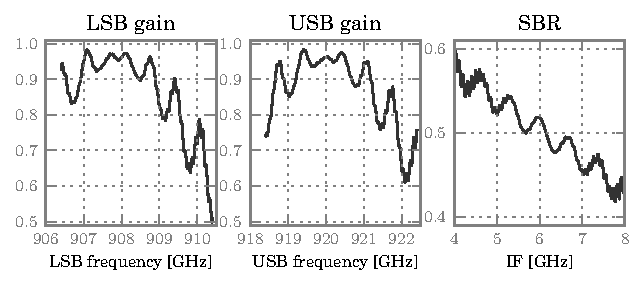
\includegraphics[scale=.9]{87_00_00_sky_s_lsbusbsbr}
        \vspace{-.8em}
        \caption{Sky signal.}
    \end{subfigure}
    \begin{subfigure}[b]{\textwidth}
        \centering
        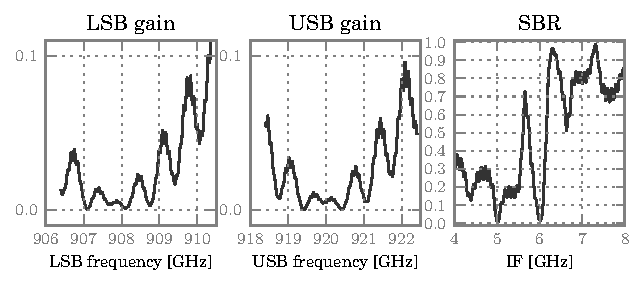
\includegraphics[scale=.9]{87_00_00_sky_l_lsbusbsbr}
        \vspace{-.8em}
        \caption{Sky local oscillator.}
    \end{subfigure}
    \begin{subfigure}[b]{\textwidth}
        \centering
        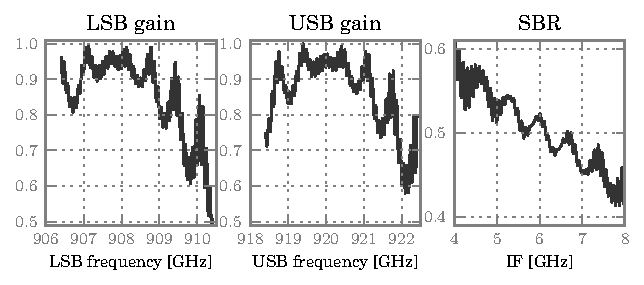
\includegraphics[scale=.9]{87_00_00_hbb_s_lsbusbsbr}
        \vspace{-.8em}
        \caption{Hot load signal.}
    \end{subfigure}
    \begin{subfigure}[b]{\textwidth}
        \centering
        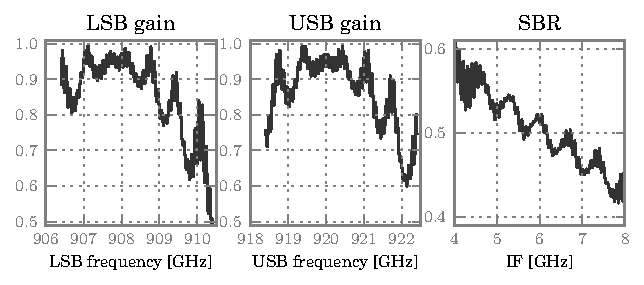
\includegraphics[scale=.9]{87_00_00_cbb_s_lsbusbsbr}
        \vspace{-.8em}
        \caption{Cold load signal.}
    \end{subfigure}
    \caption{Gain and sideband ratio of the optics for the astronomical signal~(a),
    the local oscillator noise~(b),
    the hot load~(c)
    and the cold load~(d).
    $\text{LO frequency} = \SI{914.404500}{\giga\hertz}$,
    $\text{Diplexer current} = \SI{0.503}{\milli\ampere}$.
    }
    \label{fig:87_00_00_sky_lsbusbsbr}
\end{figure}

\begin{figure}
    \centering
    \includegraphics{87_interf_usG}
    \caption{USB gain for the signal of the sky pointing, for the 95 LO and diplexer settings of the~\transition{CO}{8}{7} observation.
    Top: sorted by LO frequency then diplexer setting.
    Bottom: sorted by diplexer setting then LO frequency.}
    \label{fig:87_interf_usG}
\end{figure}
\begin{figure}
    \centering
    \includegraphics{87_interf_usB}
    \caption{USB gain for the signal of the sky pointing, divided by the bandpass, for the 95 LO and diplexer settings of the~\transition{CO}{8}{7} observation.
    Top: sorted by LO frequency then diplexer setting.
    Bottom: sorted by diplexer setting then LO frequency.}
    \label{fig:87_interf_usB}
\end{figure}

\Cref{fig:87_00_00_sky_lsbusbsbr} shows the simulated optical gain for the first spectrum of \transition{CO}{8}{7} when the chopper is pointed at the sky.
With this optical configuration, the mixer detects between~\SI{50}{\percent} and~\SI{100}{\percent} of the power of the astronomical signal and up to~\SI{10}{\percent} of the local oscillator noise.
These curves present several interesting features.
\begin{itemize}[noitemsep,nolistsep]
    \item The widest feature is a bell-shaped (or U-shaped for the LO) curve that spans the entire bandwidth.  It is a product of the diplexer.  Even a perfect diplexer performs optimally at a single frequency.  Its gain degrades as we move away from this frequency and the diplexer starts coupling the mixer to the local oscillator instead.
    \item A ripple of period~$\approx \SI{650}{\mega\hertz}$.
    This matches the length of the cavities formed by the mixers and the rooftop mirrors.
    This is caused by imperfections in the grids (they leak power to the `wrong' polarization) and the rooftop mirrors (a small fraction of the incoming power is reflected without its polarization being rotated).
    \item A ripple of period~$\approx \SI{100}{\mega\hertz}$ that is stronger at the edge of the spectrum and weaker at the center.
    This ripple is caused by the LO--mixer cavity and is modulated by the LO coupling of the diplexer.
    \item A slope in the sideband ratio, which reveals a non-optimal diplexer tuning.
\end{itemize}

The USB gain of the signal for the sky pointing (center top plot of~\cref{fig:87_00_00_sky_lsbusbsbr}) is displayed on \cref{fig:87_interf_usG} for the 95 LO and diplexer settings of the \transition{CO}{8}{7} observation.
This illustrates the influence of the LO and diplexer setting on the intensity and the phase of the ripples affecting the line, which is located at~$\approx \SI{921.8}{\giga\hertz}$.

When the chopper points to the hot or cold calibration load, the non-zero reflectivity of this load introduces more cavities in the system, which creates additional ripples to the gain curves as shown in~\cref{fig:87_00_00_sky_lsbusbsbr} (c) and (d).
The lengths of the mixer--LO, mixer--hot-load and mixer--cold-load cavities are all close to~\SI{1.5}{\meter}, and therefore all produce ripples with periods between~\num{90} and \SI{100}{\mega\hertz}.

The bandpass calibration of HIFI involves dividing the signal measured on the sky by the signal measured on the calibration loads.
The USB gain of the sky signal divided by the bandpass, as measured on the hot and cold loads, is shown in~\cref{fig:87_interf_usB}.
The comparison of~\cref{fig:87_interf_usG} and~\cref{fig:87_interf_usB} clarifies the effect of the bandpass calibration: the bell-shaped curve caused by the diplexer (red region in the center of~\cref{fig:87_interf_usG}) is canceled by the bandpass division.
In reality, the bandpass corrects more than the variable optical gain, it also corrects the frequency-dependent gain of the IF chain (the electronics between the mixer and the detector).
The cost of the bandpass calibration is the injection into the spectrum of the ripples created by interferences in the mixer--load cavities.

In order to produce these models, we have to assume values for the coefficients of reflection of the various networks of the system.
In particular, we set the reflectivity of the calibration loads to~\SI{1}{\percent} in power and that of the LO to~\SI{5}{\percent}.
The mixer reflectivity depends on the polarization: it is low in the polarization that it couples but high in the other; we choose \SI{1}{\percent} and \SI{100}{\percent}.
The wires of the grids have a radius of~\SI{1}{\micro\meter} and are separated (axis-to-axis) by~\SI{4}{\micro\meter}; their conductivity is set to~\SI{e7}{\siemens\per\meter}, the order of the conductivity of aluminum.
We assume that~\SI{2}{\percent} of the power incident on the rooftop mirrors is reflected without its polarization rotated.
Finally, we set the LO attenuation to~\SI{-6}{\decibel}.
We choose values that we think are reasonable but we expect that the spectra measured by HIFI can provide constraints on these values.

Several parameters have not been included in our simulation.
In particular, the phase of the reflection coefficients.
The reflection coefficients of the mixers and local oscillator are likely to have an imaginary part which may depend on the LO frequency: they are neither perfect conductors not perfect dielectrics.
The electronics of the local oscillator requires different settings for different LO frequencies; which change the properties of the diode on which the electromagnetic wave reflects.
Likewise, each LO setting pumps the mixers with a specific power level and we can expect the surface of a mixer to reflect differently according to its pumping.
If these imaginary parts variy quickly with frequency, then we can expect the phase and the periods of the corresponding ripples to change in accordingly.


%#############################################################################
\FloatBarrier
\section{Data reduction}
\label{sec:s140_data_reduction}
Our study focuses on spectra provided by the WBS-H backend of HIFI: the acousto-optic WideBand Spectrometer sensitive to the horizontal polarization.
The WBS allows us to see the full bandwidth of the mixers while still resolving our lines.
We choose the horizontal polarization because its system temperature is lower: in Bands~3 and 4, the V mixer is slightly under-pumped and therefore less sensitive (see~\cref{tab:chapter5_tsys}).

\begin{table}
    \centering
    \begin{tabular}{ccc}
        \toprule
        LO frequency [\si{\giga\hertz}] &
        $T_\text{sys, H}$ [\si{\kelvin}] &
        $T_\text{sys, V}$ [\si{\kelvin}]\\
        \midrule
        \num{914.46}   &   225   &   275 \\ % Tsys_1342192329 0x50003ac9
        \num{1029.52}  &   325   &   425 \\ % Tsys_1342191601 0x500037f1
        \bottomrule
    \end{tabular}
    \caption{
        System temperatures of the H and V mixers at the LO frequencies of our observation, at the intermediate frequency of our line.
        Source: Herschel Science Archive, calibration observations 0x50003ac9
        and 0x500037f1.
    }
    \label{tab:chapter5_tsys}
\end{table}


%=============================================================================

\subsection{Custom pipeline}

Because the observing mode is not standard, one assumption of the default HIFI data reduction pipeline~\parencite{hifiobserversmanual} is not valid.
It is necessary to rerun the pipeline from Level-0 (raw telemetry) to Level-2 (calibrated spectra) with a custom configuration:
the ``doAverage'' task of the pipeline must be disabled.
Leaving it enabled (the default) averages the spectra taken with different diplexer settings, which is not what we want.



%=============================================================================

\subsection{Temperature scale}
The HIFI pipeline produces spectra with a power scale expressed as an antenna temperature~$T_\text{a}$
(see~\textcite{kutner1981recommendations} for details regarding the various temperature scales used in radioastronomy).
That temperature scale is suitable for extended sources as it assumes that the emission of the source is received not only in the main beam but also in the side lobes.

\begin{figure}
    \centering
    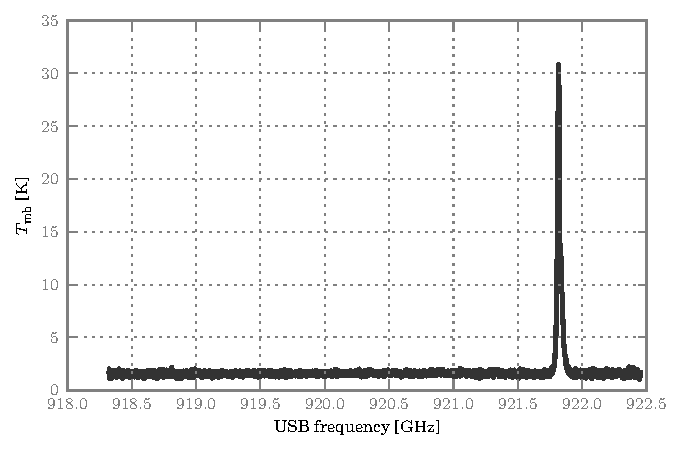
\includegraphics{87_00_00_tmb}
    \caption{
        Spectrum of \transition{CO}{8}{7} shown over its full \SI{4}{\giga\hertz} bandwidth.
    }
    \label{fig:co98_full_bandwidth}
\end{figure}

    % a = 1.22 lambda / D with D = 3.5 and lambda = c_0 / f.
    %   fl =  921.7997000e9 => ll = 0.000325225163341 => al = 0.000113364199793 rad
    %   fu = 1036.9123930e9 => lu = 0.000289120334585 => au = 0.000100779088056 rad
    % To convert to second: sec = 3600*180/pi = 206264.80624709636
    %   al * sec = 23.3830447056765
    %   au * sec = 20.78717907152951
    % To convert to diameter, multiply by distance L = 746 * parsec. (+/-4%)
    % With parsec = 3.086e16 meter
    %   al * L = 2.60982072739e+15 m  (Don't forget, 4% precision)
    %   au * L = 2.32009182242e+15 m
    % Warning, these are diameters.
    % Evgenia uses an inner radius of 2e14 cm = 2e12 m.
    % Her outer radius is 1500 times the inner radius, so 3e15.
    % That does put us pretty much exactly in that area.
    % There, she says that her density gradient for IRS1 goes as r^-0.4, calls it "mild".

Our sources are probably much smaller than our beam size and an absolute calibration of their intensity requires knowing their apparent diameter.
This does not matter for measuring our line ratios:
our two lines originate from the same regions, the ratio cancels their apparent diameter.
For our purpose, the main-beam temperature scale ($T_\text{mb}$) is appropriate.
It assumes that the source fills the main beam but not the sidelobes.

We bring the data to the main-beam temperature scale by dividing our spectra by the main-beam efficiencies $\eta_\text{mb}$ of
\num{0.744} for \transition{CO}{8}{7} and \num{0.740} for \transition{CO}{9}{8}.
We obtain these values by interpolating the beam efficiency tables attached to the HIFI observations for our LO frequencies.
%These tables have a higher granularity that the one presented in fou~\parencite{AA_537_A17}.
\Cref{fig:co98_full_bandwidth} shows one of the 95 spectra of \transition{CO}{8}{7} on the $T_\text{mb}$~scale.
%\begin{equation}
%    T_\text{mb} = T_\text{a}^* / \eta_\text{mb}
%\end{equation}

For both transitions, the \ce{CO} line is always relatively narrow ($\approx \SI{100}{\mega\hertz}$) compared to the instantaneous bandwidth of the instrument (\SI{4}{\giga\hertz}), and in the rest of this chapter we will often zoom in on the line.
The 195 spectra that we study are all very similar to the one shown in~\cref{fig:co98_full_bandwidth}.
The spectra of both transitions typically feature:
\begin{itemize}[noitemsep,nolistsep]
    \item a horizontal baseline of $\SI{1.8}{\kelvin}$ due to the difference of black-body emission at the On and the Off positions in the sky,
    \item a noise of standard deviation $\SI{0.2}{\kelvin}$ slightly stronger at the edges of the spectra than in the center.
    \item an emission line of~$\approx \SI{30}{\kelvin}$ located in the highest-frequency quarter of the spectrum.
\end{itemize}



%=============================================================================

\subsection{Diplexer mis-tuning correction}

%-----------------------------------------------------------------------------
\subsubsection{Motivation}
For our experiment, we use the diplexer as a way of modulating the interferences inside the optics of HIFI.
However, for each LO frequency there exist one and only one diplexer tuning that guarantees ideal couplings and a balanced sideband gain ratio.
By mis-tuning the diplexer, we do modulate the interferences, but we also deteriorate the sideband ratio in a way that is irrelevant for our study.
In this section, we describe how we correct for this degradation of the sideband ratio.

The diplexer units are modules of the HIFI focal plane unit that are used in Bands~3, 4, 6, and 7 for the LO injection~\parencite{jackson2002hifi}.
They are used to align the polarization of the sky and LO signals so that the mixers, which are sensitive to one polarization only, can couple to both optimally.




In normal operations, the diplexer actuator current is adjusted to the LO frequency by interpolation of a look-up table.
For our observations, we bypass this process and set the diplexer actuator current ourselves.
As a result, the diplexer is not optimally tuned.
This is illustrated in~\cref{fig:diplexer_0503}, for which the diplexer actuator current of~\SI{0.503}{\milli\ampere} for a LO frequency of~\SI{914.4045}{\giga\hertz} results in an arm length mis-tuned by \SI{158}{\micro\meter}, approximately half a wavelength.
The coupling is not symmetrical (top plot) and the sideband ratio does not equal \num{0.5} everywhere.
This distorts the line profile.
We must correct for it.

\begin{figure}
    \centering
    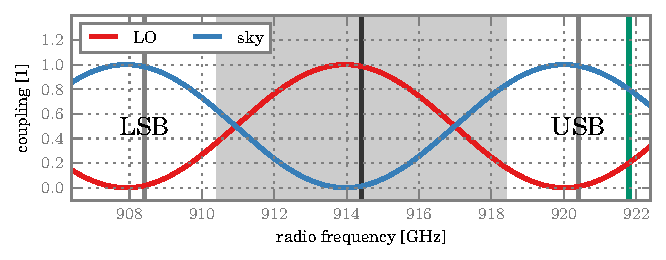
\includegraphics{diplexer_coupling_0503}
    \caption*{
        Coupling of the mixer by the LO and the sky for a mis-tuned diplexer.
        In this specific case, the coupling is shifted \SI{53}{\mega\hertz} to the left of its optimal position.
    }
    \bigskip
    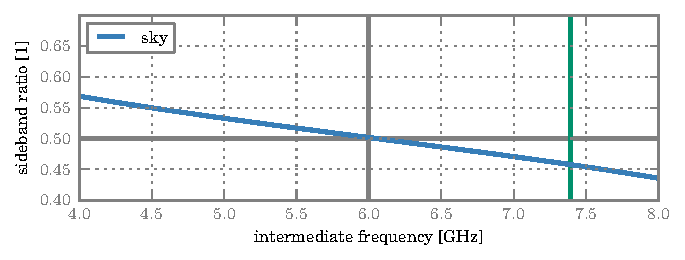
\includegraphics{diplexer_sbr_0503}
    \caption*{
        Sideband ratio of the mixer--sky coupling for a mis-tuned diplexer.
        The left part of the spectrum is USB-dominated, the right part is LSB-dominated.
        The intensity of the \transition{CO}{8}{7} line is underestimated by about~\SI{10}{\percent}.
    }
    \caption{
    Model of the coupling and the sideband ratio for a mis-tuned diplexer.
    The green vertical lines show the rest frequency of the \transition{CO}{8}{7} transition.
    The LO frequency is~\SI{914.4045}{\giga\hertz}.
    The difference in length of the two arms of the diplexer is~\SI{12.3826}{\milli\meter}.
    }
    \label{fig:diplexer_0503}
\end{figure}

%-----------------------------------------------------------------------------
\subsubsection{Correcting for the diplexer mis-tuning}
We start by assuming that the diplexer gain is the same for the four pointings of the observation (Source or On, Reference or Off, Hot, Cold):
$G_L$ for the LSB frequency and $G_U$ for the USB frequency that contribute to the same intermediate frequency.
These gains affect the powers from
the source ($S_L$ and $S_U$),
the reference ($R_L$ and $R_U$),
the hot ($H_L$ and $H_U$) and
the cold ($C_L$ and $C_U$).
The calibration equation of HIFI produces $T_\text{mb}$ from the measured powers, which are distorted by the diplexer:
\begin{equation}
    T_\text{mb}
    =
    \Delta T
    \frac{
        (G_L S_L + G_U S_U) - (G_L R_L + G_U R_U)
    }{
        (G_L H_L + G_U H_U) - (G_L C_L + G_U C_U)
    }\text{.}
\end{equation}
In this equation, $\Delta T$ is a scaling factor converting the dimensionless ratio to a temperature.
Without loss of generality, let us assume $R_L = R_U = 0$: there is no emission from the Off.

%...................................................................
\paragraph{Step 1: find the continuum.}
We assume that parts of the spectrum show only a continuum emission and no line.
Furthermore, we assume that the amplitude of the continuum is constant.
The signal in both sidebands equals this constant: $S_L = S_U = B$.
We get
\begin{equation}
    T_\text{mb}
    =
    \Delta T
    \frac{
        (G_L + G_U) B
    }{
        (G_L H_L + G_U H_U) - (G_L C_L + G_U C_U)
    }
\end{equation}
In this equation, $G_L$ and $G_U$ are known: we calculate them from a known diplexer displacement with~\cref{eq:diplexer_coupling_model}.
We also know $H$ and $C$, the emission from the hot and cold calibration loads: we know their physical temperature $T_h$ and $T_c$, their coupling coefficient and Planck's law.
Finally, $\Delta T = T_h - T_c$ is known as well.
We can therefore easily solve this equation for $B$.
Each channel of the spectrum gives a different value for $B$, but if the spectrum is flat, these values are very close to each other.
We simply take their average.

%...................................................................
\paragraph{Step 2: solve for the line.}
We know that our emission lines are located in the upper sideband.
The lower sideband sees only the continuum.
With $B$ the continuum intensity that we just calculated and $L$ the intensity of the line, we have
\begin{equation}
    T_\text{mb}
    =
    \Delta T
    \frac{
        G_L B + G_U (B + L)
    }{
        (G_L H_L + G_U H_U) - (G_L C_L + G_U C_U)
    }\text{,}
\end{equation}
which we solve for $L$.

Note: this equation cannot make the difference between the noise and the astronomical signal.
Any deviation from the baseline enters~$L$.
The intensity of the noise and the line are both `corrected' equally.

%...................................................................
\paragraph{Step 3: recalibrate.}
The previous steps give us the intensities of the continuum and the line before being distorted by the diplexer mis-tuning.
We can choose whether we re-introduce the continuum or if we leave it out.
The two situations are described by the equations
\begin{align}
    T_\text{mb}'
    &=
    \Delta T
    \frac{B+L}{(H_L + H_U) - (C_L + C_U)} \text{\quad with continuum and}
    \\
    T_\text{mb}''
    &=
    \Delta T
    \frac{L}{(H_L + H_U) - (C_L + C_U)} \text{\quad with the line only.}
\end{align}

In the rest of this chapter, we use the $T_\text{mb}''$ scale.

%-----------------------------------------------------------------------------
\subsubsection{Result of the diplexer mis-tuning correction}
\Cref{fig:diplexer_correction} shows the result of correcting the sideband imbalance with this simple method.
The bottom plot for each transition shows the line only, the continuum is removed.

\begin{figure}
    \centering
    \begin{subfigure}[b]{\textwidth}
        \centering
        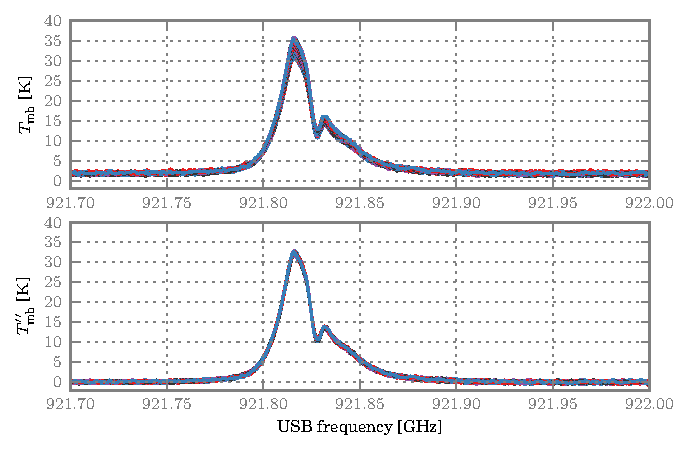
\includegraphics{correction_87}
        \vspace{-.8em}
        \caption{\transition{CO}{8}{7} spectra before and after sideband correction.}
    \end{subfigure}
    \\
    \bigskip
    \begin{subfigure}[b]{\textwidth}
        \centering
        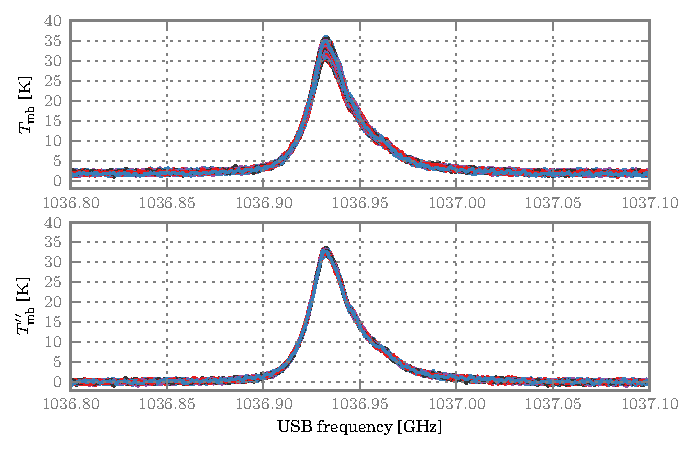
\includegraphics{correction_98}
        \vspace{-.8em}
        \caption{\transition{CO}{9}{8} spectra before and after sideband correction.}
    \end{subfigure}
    \caption{
        Correction of the sideband imbalance due to mis-tuning the mixer.
    }
    \label{fig:diplexer_correction}
\end{figure}


For both transitions, the spread of the peak intensity is considerably reduced.
\begin{table}
    %87 Before correction 31.5146912873 +/- 1.31935031215
    %87 After  correction 32.3597611286 +/- 0.27093631469
    %98 Before correction 31.2396155249 +/- 1.49534099289
    %98 After  correction 32.7454980568 +/- 0.448444802488
    \centering
    \begin{tabular}{ccc}
        \toprule
        transition & before correction & after correction \\
        \midrule
        \transition{CO}{8}{7} & $\num{31.5} \pm \SI{1.3}{\kelvin}$ &
                                $\num{32.4} \pm \SI{0.3}{\kelvin}$\\
        \transition{CO}{9}{8} & $\num{31.2} \pm \SI{1.5}{\kelvin}$ &
                                $\num{32.7} \pm \SI{0.5}{\kelvin}$\\ 
        \bottomrule
    \end{tabular}
    \caption{Peak intensities before and after correcting for the diplexer mis-tuning.}
\end{table}

Any residual spread is due to either thermal noise, imperfections in the diplexers and interferences in the optics.





%#############################################################################
%\FloatBarrier
\section{Noise simulations}
\label{sec:noise_simulations}
We wish to quantify the influence of the thermal noise on the line profiles.
We model the noise seen on HIFI observations and use that model to generate synthetic spectra.
This mimics an observation in which the same source is observed many times with a fixed LO and diplexer settings.
These synthetic spectra differ only by their noise, not by variations in the optical gain.
We proceed in three steps.
First, construct an ideal spectrum for each transition.
Then, model the thermal noise affecting the real spectra.
Finally, apply the modeled thermal noise to the ideal spectra.



%=============================================================================

\subsection{Ideal spectra}
For our ideal hopefully-noiseless spectra, we choose to average the 95~spectra of each transition.
The averaged spectra are shown in~\cref{fig:corrected_averaged}.
We do not claim that these averaged spectra are closer to the astronomical reality than any individual spectrum: averaging reduces the noise but may leave systematic instrumental effects in the bandpass.

By averaging, we reduce the noise by a factor~$\sqrt{95} \approx 10$ but we do not completely eliminate it.

\begin{figure}
    \centering
    \begin{subfigure}[b]{\textwidth}
        \centering
        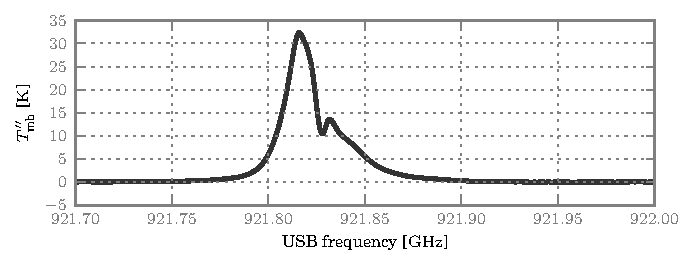
\includegraphics{87_avera_corrected_tmb}
        \vspace{-.8em}
        \caption{Average of the 95 \transition{CO}{8}{7} diplexer-corrected spectra.}
    \end{subfigure}
    \\
    \begin{subfigure}[b]{\textwidth}
        \centering
        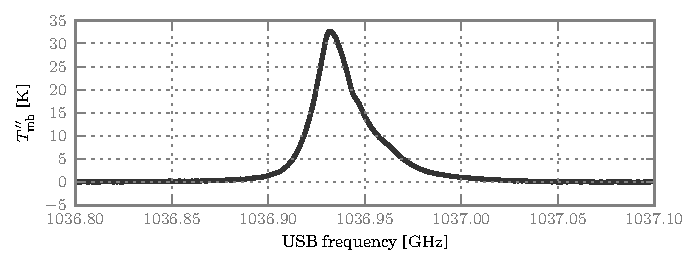
\includegraphics{98_avera_corrected_tmb}
        \vspace{-.8em}
        \caption{Average of the 95 \transition{CO}{9}{8} diplexer-corrected spectra.}
    \end{subfigure}
    \caption{Average of the spectra corrected for diplexer mix-tuning.}
    \label{fig:corrected_averaged}
\end{figure}

%=============================================================================
\subsection{Thermal noise modeling}
We model the thermal noise with a polynomial in Fourier space.

Using Fourier Transforms to analyze a signal is relatively trivial: signals have an analytic expression, they can be written as function of time or frequency.
The noise does not have an analytic expression: it is a stochastic process that can be described only in statistical terms such as variance.
The noise is not visible on the spectra that we measured, what we have is one very specific instance of an inherently random process, one single state taken out of the infinite%
\footnote{Infinite if we assume that the probability distribution is continuous, but quantum processes ultimately limit this to a finite, albeit overwhelmingly large, state space.}
state space of the system.
Fourier analysis treats that particular state as if it were signal.
We must estimate the properties of the stochastic process from that specific sequence.

The power of a stochastic process is, in statistical term, its variance.
The variance can be a function of frequency, for example the ``pink noise'' or the ``$1/f$ noise'' have different variances at different frequencies.
These can be represented on a ``periodogram'', a graph that plots the ``power spectral density'' (PSD) as a function of a frequency/period/scale.
If we consider a time-varying electric potential in volt,
the unit of the PSD of its noise is \si{\volt\squared\second} or \si{\volt\squared\per\hertz}.
In our case, the data is a temperature as a function of frequency;
the PSD of its noise is in~\si{\kelvin\squared\hertz}.
The estimation of the PSD from a signal is a subtle matter, subject of a significant volume of literature (i.e.\ \textcite{burg1967maximum,percival1993spectral}).

In our situation, an accurate estimation of the PSD is not required.
Our goal is to generate 190~synthetic spectra which present 190~particular noise states.
It is sufficient to know these 190~particular states, one does not need to model accurately the entire state space.
We only need the Fourier Transform of our synthetic spectra to match that of the real data.

Taking spectra of spectra can lead to a confusing terminology.
Furthermore there are at least four Fourier spectra of interest for a single direct spectrum.
\Cref{tab:direct_fourier} clarifies the terminology used in this section.

\begin{table}
    \centering
    \begin{tabular}{llcll}
    \toprule
    \multicolumn{5}{l}{Direct spectrum}\\
    \midrule
    $x$-axis & frequency   & $f$ & $\mathbb{R}$ & [\si{\hertz}]\\
    $y$-axis & temperature & $T$ & $\mathbb{R}$ & [\si{\kelvin}]\\
    \bottomrule
    \\
    \toprule
    \multicolumn{5}{l}{Fourier spectra}\\
    \midrule
    $x$-axis & reciprocal frequency & $t$         & $\mathbb{R}$ & [\si{\per\hertz}]\\
    $y$-axis & complex spectrum     & $z$         & $\mathbb{C}$ & [\si{\kelvin}]   \\
             & phase spectrum       & $\arg(z)$   & $\mathbb{R}$ & [\si{\radian}]   \\
             & amplitude spectrum   & $\abs{z}$   & $\mathbb{R}$ & [\si{\kelvin}]   \\
             & normalized-amplitude spectrum & $\abs{z}/n$& $\mathbb{R}$ & [\si{\kelvin}]   \\
    \bottomrule
    \end{tabular}
    \caption{Definitions and units used in Direct and Fourier space.}
    \label{tab:direct_fourier}
\end{table}

Normalized amplitudes allow the comparison of spectra taken with different sampling rates~$\delta f$ and/or different bandwidths~$\Delta f = n \delta f$ (with $n$ the number of channels in the spectrum) by multiplying them by $\delta f / \Delta f = 1/n$.
We use amplitude and normalized-amplitude spectra where necessary:
amplitude spectra can be converted back to direct space;
normalized-amplitude spectra can be compared.

We do not analyze our noise with energy density or power density spectra.
Energy and power density spectra require raising the amplitude to the power 2, which enhances the contrast between the high- and low-amplitude parts of the spectra.
From our experiments, we determined that fitting the energy or power spectrum requires a polynomial of order $>10$ while an order-6 is sufficient to fit the amplitude.
Furthermore, we need our final result in amplitude so that it can be converted back to the direct domain with an inverse-DFT, making the round-trip between amplitude and power unnecessary.

It is easier to measure the noise on the the baseline than on the lines.
The lines are located in the high-frequency half of the direct spectra (see~\cref{fig:co98_full_bandwidth}), therefore we take the Fourier Transform of the lower-frequency half.
We remove any continuum level from the direct spectrum to minimize the artifacts created by the Discrete Fourier Transform (DFT) algorithm.

Finally, we do not apodize our direct spectra with a window.
Windowing is recommended to reduce the ``leakage'' caused by the truncation of the direct data when we need to accurately quantify the amplitude/energy/power at a given frequency on a correct scale.
We are not interested in the absolute levels of amplitude/energy/power;
we are satisfied when the normalized-amplitude of the synthetic spectrum matches that of the real spectrum, leakage included.

%-----------------------------------------------------------------------------
\subsubsection{Noise model of the ideal spectra}

The noise spectra of our ideal spectra are shown in \cref{fig:noise_model_87}(a)
and~\cref{fig:noise_model_98}(a).
The normalized amplitude is in black and its polynomial model in red.

The small plots inside the larger ones zoom into the region in which we expect interferences to leave traces.
Their $x$-axis gives the period of the ripples caused by interferences.
These spectra peak at two periods:
$\approx\SI{90}{\mega\hertz}$ and $\approx\SI{600}{\mega\hertz}$.

The $\SI{90}{\mega\hertz}$ ripple originates from the mixer--LO, mixer--hot-load and/or mixer--cold load cavities.
These cannot be distinguished at this resolution.

The $\SI{600}{\mega\hertz}$ ripple comes from the mixer--rooftop-mirrors cavities.

The averaging process by which we create the ideal spectra retains these two ripples.
This indicates that their phase varies little over the 95~spectra involved in the average:
they interfere constructively.

The polynomial model ignores these peaks of amplitude density: these regions are deliberately masked before fitting the polynomial.
Indeed, the polynomial must follow the thermal noise only and these peaks are not of thermal origin.

%-----------------------------------------------------------------------------
\subsubsection{Noise model of the real spectra}
\label{sec:noise_model_of_the_real_spectra}

The main sources of noise in HIFI are the mixer, the local oscillator and the telescope dish.
The diplexer setting has an influence on how much LO noise the mixer receives but we calculate that our diplexer settings should change that value by less than one percent.
The LO is responsible for less than~\SI{10}{\percent} of the total system temperature.
We conclude that, for modeling our noise, we should not attempt to ``correct'' its intensity for diplexer mis-tuning.
The noise measured on the original spectra is the correct one.

In this step, we do not take the DFT of an average but the average of DFTs.
Indeed, we do not wish to attenuate the noise of the real spectra by averaging them.
However, we wish to reduce the uncertainty of our polynomial model, which we can achieve by averaging the DFTs.

The normalized-amplitude spectra of the baseline, and their polynomial models, are presented in~%
\cref{fig:noise_model_87}(b) and~\cref{fig:noise_model_98}(b).

The two peaks at~\SI{90}{\mega\hertz} and~\SI{600}{\mega\hertz} that are present on the ideal spectra are also visible on these real spectra.
These peaks are less well-defined because the noise is stronger.

A new feature appears on these spectra: a peak at~\SI{875}{\per\giga\hertz} which corresponds to a period of~$\approx\SI{1.14}{\mega\hertz}$.
This peak is visible on the average of DFTs but not on the DFT of averages.
This indicates that the corresponding ripple interferes destructively during the averaging: its phase changes a lot.
It is unlikely that this feature corresponds to a cavity: the cavity would need to be~\SI{130}{\meter}-long.
We have not determined its origin.
Possible explanations include
\begin{itemize}[noitemsep,nolistsep]
    \item An artifact of the sampling of the WBS:
the even and odd channels of the WBS CCD have different levels of dark currents.
These channels are separated by about~\SI{0.5}{\mega\hertz} and an imperfect calibration of these dark currents could generate a~\SI{1}{\mega\hertz}-period ripple.
    \item An artifact of the regridding done by the HIFI pipeline:
the spectra produced by the WBS have an irregular frequency axis.
The pipeline resamples it onto a regular grid.
This might produce some artifacts at the scale of the channel spacing (\SI{0.5}{\mega\hertz}) or the channel resolution~\SI{1.1}{\mega\hertz}.
\end{itemize}
In any case, this feature is non-thermal and its region is masked during the fit of our polynomial model.

\begin{figure}[p]
    \centering
    \begin{subfigure}[b]{\textwidth}
        \centering
        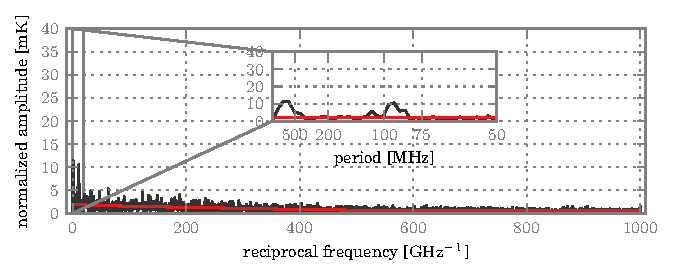
\includegraphics{noise_dft_87_correctedavg}
        \vspace{-.8em}
        \caption{Noise of the average of 95 \transition{CO}{8}{7} diplexer-corrected spectra.}
        %\label{fig:noise_dft_87_correctedavg}
    \end{subfigure}
    \\
    \bigskip
    \begin{subfigure}[b]{\textwidth}
        \centering
        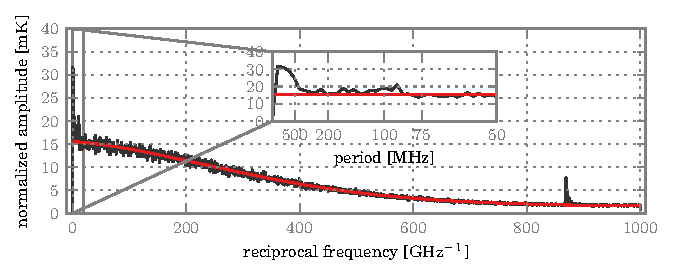
\includegraphics{noise_dft_87_original}
        \vspace{-.8em}
        \caption{Averaged noise of 95 \transition{CO}{8}{7} original spectra.}
        %\label{fig:noise_dft_87_original}
    \end{subfigure}
    \\
    \bigskip
    \begin{subfigure}[b]{\textwidth}
        \centering
        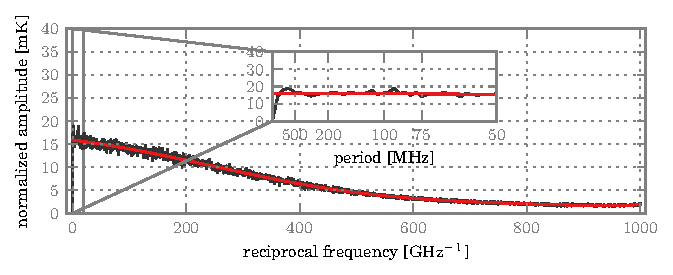
\includegraphics{noise_dft_87_noisy}
        \vspace{-.8em}
        \caption{Averaged noise of 95 \transition{CO}{8}{7} synthetic noisy spectra.}
        %\label{fig:noise_dft_87_noisy}
    \end{subfigure}
    \caption{Noise modeling of the~\transition{CO}{8}{7} spectra.}
    \label{fig:noise_model_87}
\end{figure}

\begin{figure}[p]
    \centering
    \begin{subfigure}[b]{\textwidth}
        \centering
        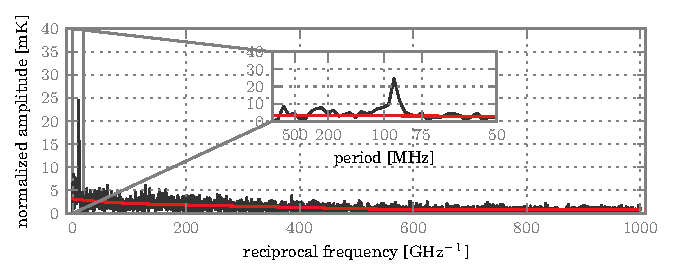
\includegraphics{noise_dft_98_correctedavg}
        \vspace{-.8em}
        \caption{Noise of the average of 95 \transition{CO}{9}{8} diplexer-corrected spectra.}
    \end{subfigure}
    \\
    \bigskip
    \begin{subfigure}[b]{\textwidth}
        \centering
        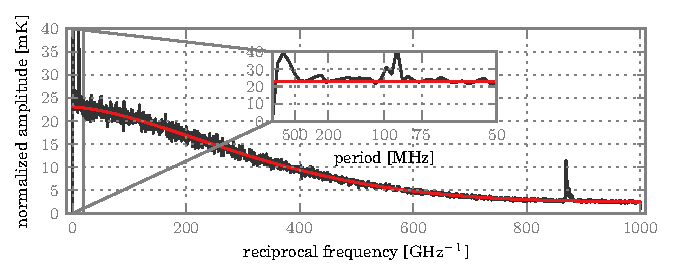
\includegraphics{noise_dft_98_original}
        \vspace{-.8em}
        \caption{Averaged noise of 95 \transition{CO}{9}{8} original spectra.}
    \end{subfigure}
    \\
    \bigskip
    \begin{subfigure}[b]{\textwidth}
        \centering
        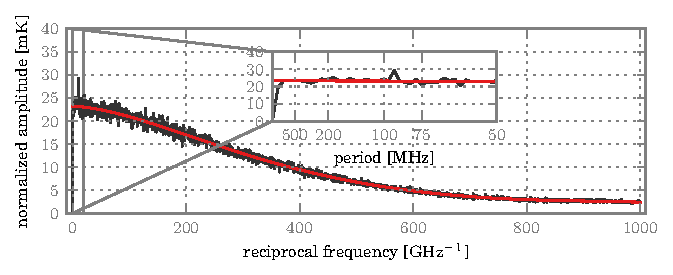
\includegraphics{noise_dft_98_noisy}
        \vspace{-.8em}
        \caption{Averaged noise of 95 \transition{CO}{9}{8} synthetic noisy spectra.}
    \end{subfigure}
    \caption{Noise modeling of the~\transition{CO}{9}{8} spectra.}
    \label{fig:noise_model_98}
\end{figure}


%=============================================================================
\FloatBarrier
\subsection{Synthesis of the thermal noise}
We generate artificial noise in the Fourier space and convert it to Direct space with an inverse Discrete Fourier Transform via a technique called ``phase randomization'' \parencite{yamada1991orthonormal}.

The complex spectrum of our synthetic noise is an array of complex numbers $z=\rho \exp(i \theta)$.
The array $\rho=\abs{z}$ is an amplitude spectrum.
The array $\theta=\arg(z)$ is a phase spectrum.

A polynomial model describes a normalized-amplitude spectrum $\abs{z}/n$ with $n$ the number of channels.
Multiplying that model by the appropriate $n$ gives a amplitude spectrum $\rho$.

We use a pseudo-random number generator with a uniform distribution to generate a phase spectrum with values of $\theta \in [0, 2\pi[$.

We call $A$ the noise model of the ideal spectra and $B$ the noise model of the real spectra.
The noise that we need to add to the ideal spectra in order to bring them to $A$ is not
$C=A-B$: noise adds in power, not in intensity.
The addition in power ($C=\sqrt{A^2-B^2}$) does not produce synthetic spectra with a noise of $A$ either: the randomness is too high (or the number of channels too low).
Instead, we determine $C$ by fitting it; the objective function generates hundreds of synthetic spectra at each iteration until the normalized-amplitude spectrum of their noise matches~$A$.

The average noise of our 190 synthetic spectra (95 per transition) can be seen
in~\cref{fig:noise_model_87}(c) and~\cref{fig:noise_model_98}(c).
As desired, it is very similar to the noise observed on the real spectra (middle plots).
In addition, the peaks present on the top and middle spectra have all but disappeared.

We have created synthetic spectra that mimic the noise seen on the real spectra without including their systematic variability.
We can now analyze the line profiles of the real and synthetic spectra.




%#############################################################################
\FloatBarrier
\section{Line profile analysis}



We begin our analysis by measuring the various components constituting the lines profiles of \transition{CO}{8}{7} and \transition{CO}{9}{8} seen by HIFI in S140 IRS1.

We perform the same analysis with two sets of spectra:
the real HIFI spectra corrected for diplexer-mis-tuning (\cref{sec:s140_data_reduction})
and
the synthetic spectra that simulate an observation that is affected only by thermal noise (\cref{sec:noise_simulations}).


%=============================================================================
\FloatBarrier
\subsection{Gaussian model of the spectra}
\label{sec:chp5_gaussian_model}
\Cref{fig:spectra_transitions} shows the real diplexer-corrected spectra for an arbitrary LO and diplexer setting, one for each transition.
Superimposed on these spectra are the various components of a model.

\begin{figure}
    \centering
    \begin{subfigure}[b]{\textwidth}
        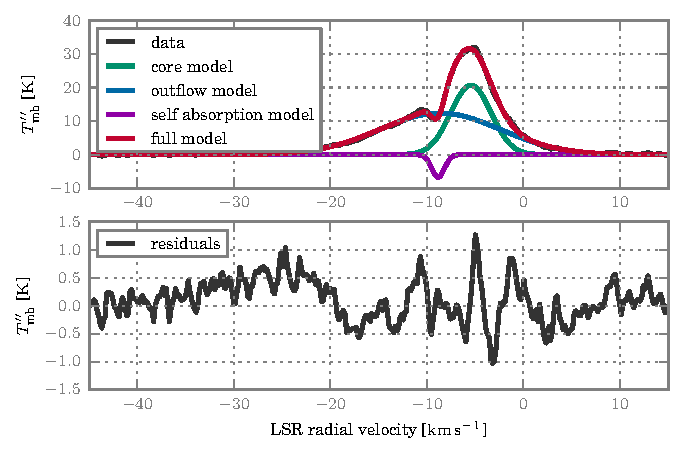
\includegraphics{87_00_00_corrected}
        \vspace{-.8em}
        \caption{\transition{CO}{8}{7}, rest frequency \SI{ 921.7997000}{\giga\hertz}.}
    \end{subfigure}
    \\
    \bigskip
    \begin{subfigure}[b]{\textwidth}
        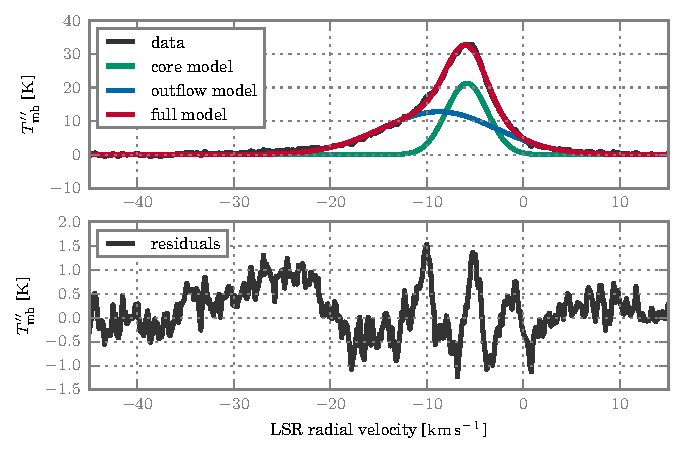
\includegraphics{98_00_00_corrected}
        \vspace{-.8em}
        \caption{\transition{CO}{9}{8}, rest frequency \SI{1036.9123930}{\giga\hertz}.}
    \end{subfigure}
    \caption{
        HIFI WBS-H spectra of S140 IRS1 for \transition{CO}{8}{7} and \transition{CO}{9}{8}.
        For each transition, the the top plot shows the data in black and the model in color, where the full model is the sum of the others; and the bottom plot shows the difference between the data and the full model.
    }
    \label{fig:spectra_transitions}
\end{figure}

The model is composed of three or four elements:
\begin{itemize}[noitemsep,nolistsep]
    \item a constant horizontal continuum ($c$),
    \item a narrow Gaussian for the core emission ($a_0$, $v_0$, $\sigma_0$),
    \item a broad Gaussian for the outflow emission ($a_1$, $v_1$, $\sigma_1$),
    \item and optionally a third negative Gaussian for a self-absorption component
     ($a_2$, $v_2$, $\sigma_2$).
\end{itemize}
Both transitions show a self-absorption, but in the case \transition{CO}{9}{8} the self-absorption is barely visible in the noise, which makes it difficult to fit.
For each Gaussian function, $a$ is the amplitude, $v$ the mean and $\sigma$ the standard deviation.

%-----------------------------------------------------------------------------
\subsubsection{Core and outflow velocity}
The outflow is not as collimated as the jet that creates it; shocks, collisions and turbulence create a wide range of velocities inside the outflow.
In comparison, the velocities in the core are more homogeneous.
Through the Doppler effect, a larger velocity range translates into broader lines, which is why the outflow component (blue in~\cref{fig:spectra_transitions} is wider than the core component (in green).

The \ce{CO} lines of S140~IRS1 are blue-shifted;
the core moves towards us with a radial velocity of~\SI{-5}{\kilo\meter\per\second}.
The peak intensity of the outflow is on the blue side of the core: it approaches us at~\SI{-9}{\kilo\meter\per\second}, faster than the core does.
\Textcite{maud2013s140} measure a speed of~\SI{-25}{\kilo\meter\per\second} for the blue \transition{CO}{1}{0} outflow.
We justify the difference by the distance to the core.
Our high-$J$ lines are emitted near the core, the jet had little time to accelerate the \ce{CO} molecules.
On the other hand, the \transition{CO}{1}{0} outflow is observed much farther and has been accelerated by the jet much longer.

The line profiles do not show any evidence of a bimodal distribution of velocities as one could expect from a rotating disk seen edge-on.
We conclude that the emission that we observe does not originate (solely) from the accretion disk orbitting the young stellar object.

%-----------------------------------------------------------------------------
\subsubsection{Missing red outflow}
Since the outflow of IRS1 is bipolar, one would expect a second outflow line on the red side of the core.
The spectra do not show this second outflow component.
The emission of the red outflow
may be weaker due do different density and temperature conditions
or it may be absorbed by the dense circumstellar envelope before reaching the detector.

%-----------------------------------------------------------------------------
\subsubsection{Self-absorption}
The absorption feature seen at~$v_\text{LSR}=\SI{-9}{\kilo\meter\per\second}$ attests that \transition{CO}{8}{7} is not optically thin at all frequencies.
The absorption and outflow components have a similar velocity:
this is a case of self-absorption, in which the photons at the line wings have a smaller re-absorption probability than the photons at the line center.

%-----------------------------------------------------------------------------
\subsubsection{Structure of the residual}
The difference between the data and our model (``residuals'' on the plots) shows some structure.
In particular, the blue wing of the line is systematically underestimated: the residual at~\SI{-25}{\kilo\meter\per\second} reaches~\SI{0.5}{\kelvin}.
We have attempted to model the outflow with a second Gaussian component in the hope that it would reveal an emission from the red outflow and increase the velocity of the blue one.
These attempts were unsatisfactory: the models converged to an ad-hoc solution that fitted the blue tail with a very wide and flat Gaussian and showed no evidence of emission from the red outflow.

The three peaks in the residual show that Gaussian profiles are not a perfect fit for this spectrum.
This structure may be astronomical or it can be an instrumental artifact.

\begin{figure}[b!]
    \centering
    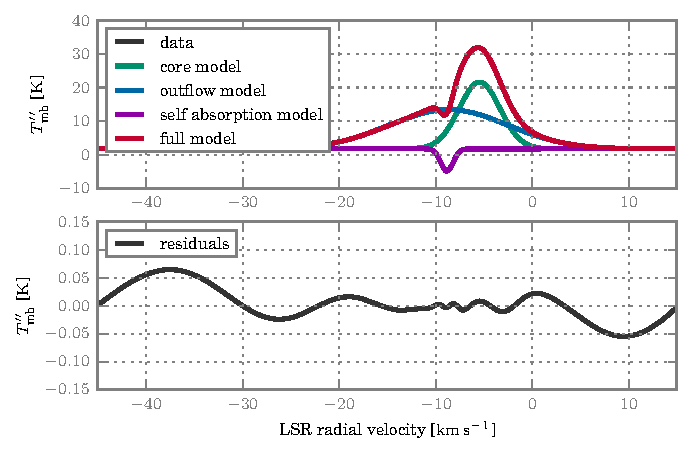
\includegraphics{87_00_00_interf}
    \caption{
        Interference model of HIFI Band~3 applied to a perfectly Gaussian source.
        The interferences introduce ripples the spectrum.
        A Gaussian model of this spectrum leaves a residual that shows some ripples.
    }
    \label{fig:87_00_00_interf}
\end{figure}

We apply the interference model of Band~3 from~\cref{sec:s141_interf} to an input that is made of three perfect Gaussian.
The result is shown in~\cref{fig:87_00_00_interf}.
The interferences modulate the gains and create ripples on the spectrum, which appear on the residual of its Gaussian model.


The small-scale structure located at the frequencies on the line could correspond to that seen on the real spectra, only with a different intensity.
If the real small-scale structure is caused by interferences, then our interference model underestimates them, at least for this specific LO and diplexer setting.

The large-scale structure that modulates the wings of the line does not match that of the real spectra: the interference model creates a long negative red tail that does not exist in the real spectra.
Here, our interference model overestimates the amplitude of that ripple.

It is unlikely that the residual structure is solely caused by interferences in the optics.
Wavelet analysis (\cref{fig:wavelet}) indicates that the periods of the residual structure do not match that of the ripples caused by interferences in known cavities.
They do not match harmonics of these ripples either, harmonics which are anyway unlikely to matter because of the low reflection coefficients in the cavities.
\Cref{fig:wavelet} shows only two scaleograms out of 190.
These scaleograms vary greatly from one spectrum to another.
Most reveal traces of the expected ripple at~\SI{640}{\mega\hertz} that originates from the mixer--rooftop-mirrors cavities, but the indication of a ripple of period between~\num{90} and \SI{100}{\mega\hertz} centered on the line is unclear.

\begin{figure}[p]
    \centering
    \begin{subfigure}[b]{\textwidth}
        \centering
        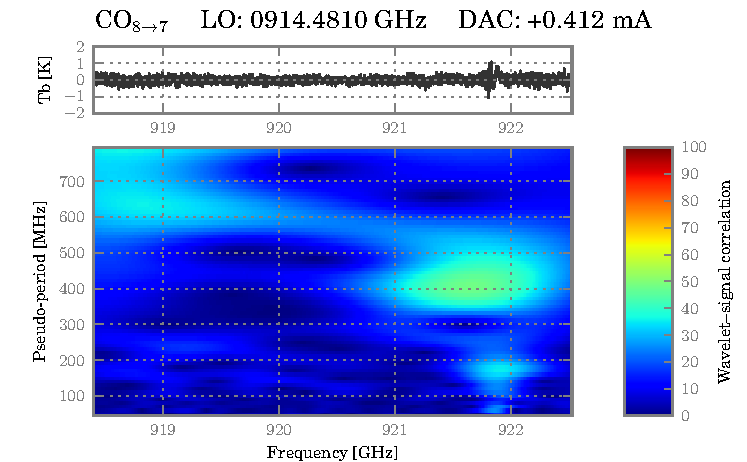
\includegraphics[width=\textwidth]{50015e1d_WBS-H-USB_04-16_fit_wavelet}
    \end{subfigure}\\
    \begin{subfigure}[b]{\textwidth}
        \centering
        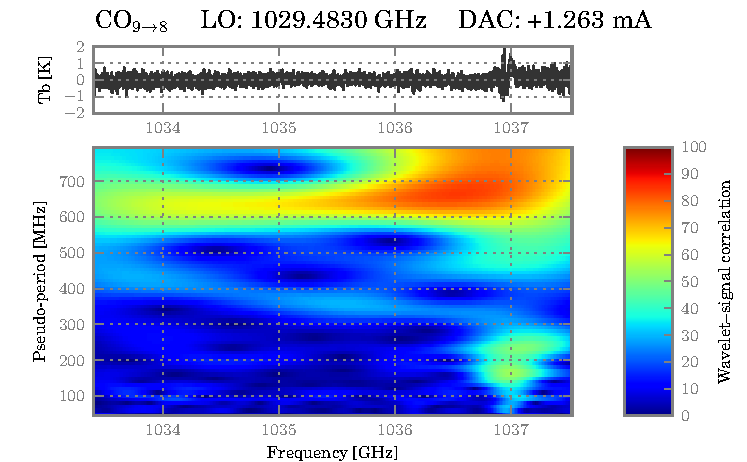
\includegraphics[width=\textwidth]{50015d89_WBS-H-USB_00-12_fit_wavelet}
    \end{subfigure}
    \caption{
        Scaleogram of the continuous wavelet transform
        of the residual of two spectra after subtraction of their Gaussian model.
        The wavelet used is a Morlet wavelet with a time/frequency compromise of 10.
        Colors fade on the edges due to the wavelet sampling 0 outside the defined spectrum.
    }
    \label{fig:wavelet}
\end{figure}

Consequently, we claim that the structure that we observe on the residual of the Gaussian fit of our HIFI spectra is, at least in part, of astronomical nature: the observed emission is not Gaussian.




%-----------------------------------------------------------------------------
\subsubsection{Summary}
The geometry of IRS1 presented by~\textcite{maud2013s140} is that of a source seen almost edge-on: a central object circled by an accretion disk that appears very elliptic (elongated in the NE-SW direction), and two large \transition{CO}{1}{0} outflows perpendicular to the disk (SE is blue-shifted, slightly in front of the core, NE is red-shifted, slightly behind the core).
Our HIFI observation of high-$J$ \ce{CO} lines show a different picture: only the blue outflow is visible as one would expect in the case of a face-on geometry.

Both views can be reconciled if we assume that the system is seen almost edge-on but has a dense circumstellar envelope.
The slight inclination of the polar axis is sufficient to cause the extinction of the red outflow but not that of the blue one, which we would not expect from a homogeneous system.
This suggests a considerable increase of the column density of~\ce{CO} caused by a dense layer of gas between the two outflows, which is compatible with the strong density gradient that we expect close to the central object.
If our high-$J$ \ce{CO} lines originate very close to the center of the system,
the envelope absorbs the emission of the red outflow.

Our lines are not everywhere optically thin, as demonstrated by the visible self-absorption on the blue outflow and the total absence of visible red outflow.
This skews the lines profiles.
Our Gaussian models fit them imperfectly, which can explain the structure of the residual.
In addition, interferences in the optics of the instrument can bring additional distortions to the line profiles.


%=============================================================================
\FloatBarrier
\subsection{Line statistics}
We apply the Gaussian model described in the previous section to the 190 spectra of our observation and the 190 synthetic spectra.
With a least-square Levenberg-Marquardt algorithm, we fit the parameters
$c$,
$a_0$, $v_0$, $\sigma_0$,
$a_1$, $v_1$, $\sigma_1$, and optionally
$a_2$, $v_2$ and $\sigma_2$, for each spectrum independently.

From these fits, we can derive velocity-integrated intensities, then velocity-integrated intensity ratios.

%-----------------------------------------------------------------------------
\subsubsection{Gaussian model parameters}

\Cref{fig:fit_core_87,fig:fit_core_98,fig:fit_outf_87,fig:fit_outf_98,fig:fit_sabs_87,fig:fit_base} present the fitted parameters.
The horizontal axis of each plot corresponds to the spectrum number.
There are 95 spectra for each transition, therefore 95 points on each plot.
The spectra are ordered by LO frequency first (slow-moving index), then by diplexer setting (fast-moving index).

For the Gaussian components, we plot the Full Width at Half Maximum (\textsc{fwhm}) instead of the standard deviation $\sigma$, for its interpretation as a line width is more visual and intuitive; both quantities are linked by
\begin{equation}
    \textsc{fwhm} = 2 \sigma \sqrt{2 \ln(2)}\text{.}    \label{eq:fwhm_sigma}
\end{equation}

The error bars on these plots are fitting errors.
They are calculated by multiplying the diagonal of the covariance matrix by the noise variance (assumed to be that of the baseline) and taking its square root.

When the amplitude and the standard deviation of a Gaussian are known, it is easy to compute the area under that Gaussian, called ``integrated intensity'':
\begin{equation}
    \int_{-\infty}^{+\infty} a \mathrm{e}^{- \frac{(x-v)^2}{2 \sigma^2}}\,\mathrm{d}x
    =
    a \abs{\sigma} \sqrt{2\pi}
    \text{.}
    \label{eq:gaussian_integral}
\end{equation}
We integrate the Gaussian models of the lines over all velocities to produce velocity-integrated intensities in~\si{\kelvin \kilo\meter\per\second}.

The amplitude of the core components for both transitions (\cref{fig:fit_core_87,fig:fit_core_98}) presents some structure:
they cluster around different values for each LO frequency.
The same is true for the amplitude the~\transition{CO}{9}{7} outflow.
The \transition{CO}{8}{7} outflow seems to follow a linear trend, which may be a particular case of the clustering seen on the other plots.
Obviously the LO frequency influences the sideband ratio in ways that our diplexer mis-tuning correction does not predict.
Within a LO frequency, however, the effect of the diplexer is almost drowned in the noise.

In~\cref{sec:s141_interf} we simulated the interferences in optics of HIFI for values that we considered ``reasonable''.
In particular, we used coefficients of reflection that are particularly low: only~\SI{1}{\percent} in power, which means that a single round trip in a cavity results in an attenuation by $0.0001$.
Despite these low reflections, our interference model predicts ripples that are stronger than the ones observed on our data.
Nevertheless, we cannot claim that the reflection coefficients that we used in our model are too high:
when the mixer folds the LSB gain on top of the USB gain, the LSB ripple interferes with the USB ripple (\cref{fig:lo_scan_of_ripple}).
The amplitude and phase of the LSB and USB ripples become degenerated when folded.
Strong ripples can interfere destructively with themselves and weak ripples can interfere constructively.
As a result, we lack constraints to properly model the interferences in the optics of HIFI.



\begin{figure}[b]
    \centering
    \begin{tabular}{@{}c@{}c@{}}
    \toprule
        \multicolumn{2}{c}{\transition{CO}{8}{7} continuum} \\
        diplexer-corrected & synthetic                 \\
    \midrule
        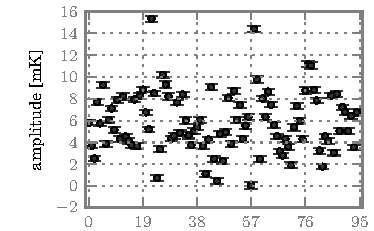
\includegraphics{spread_87_base_ampl_corrected}&
        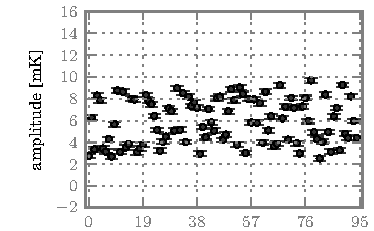
\includegraphics{spread_87_base_ampl_noisy}        \\
    \bottomrule
    \toprule
        \multicolumn{2}{c}{\transition{CO}{9}{8} continuum} \\
        diplexer-corrected & synthetic                 \\
    \midrule
        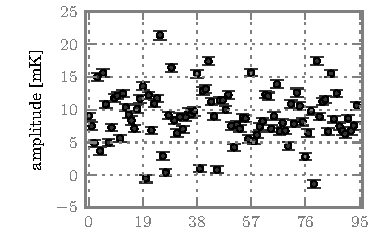
\includegraphics{spread_98_base_ampl_corrected}&
        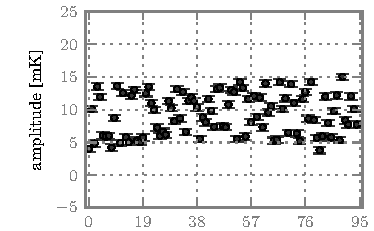
\includegraphics{spread_98_base_ampl_noisy}            \\
    \bottomrule
    \end{tabular}
    \caption{
        Continuum fitted on the real (left) and synthetic (right) spectra for the two transitions.
    }
    \label{fig:fit_base}
\end{figure}

%\afterpage{% Make sure the two figures appear on even/odd pages for comparison.
%    \clearpage% flush all other floats
%    \ifodd\value{page}
%    %\else% uncomment this else to get odd/even instead of even/odd
%        \expandafter\afterpage% put it on the next page if this one is odd
%    \fi
%    {%
    \begin{figure}[p]
        \centering
        \begin{tabular}{@{}c@{}c@{}}
            \toprule
            \multicolumn{2}{c}{\transition{CO}{8}{7} core} \\
            diplexer-corrected & synthetic                 \\
            \midrule
            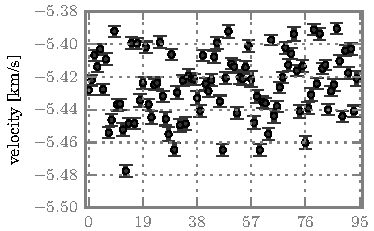
\includegraphics{spread_87_core_velo_corrected}&
            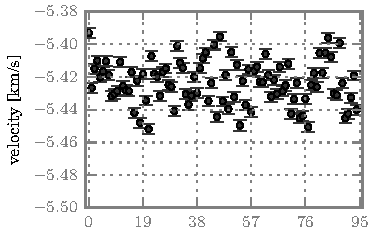
\includegraphics{spread_87_core_velo_noisy}    \\
            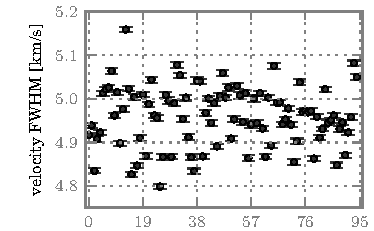
\includegraphics{spread_87_core_vfwh_corrected}&
            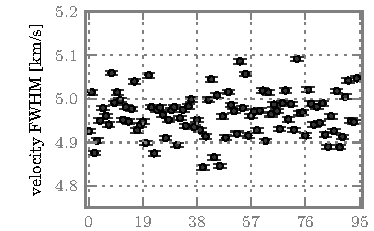
\includegraphics{spread_87_core_vfwh_noisy}    \\
            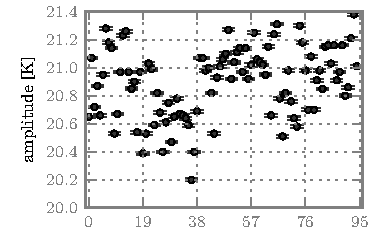
\includegraphics{spread_87_core_ampl_corrected}&
            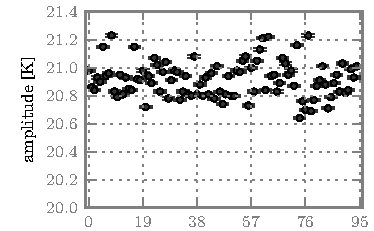
\includegraphics{spread_87_core_ampl_noisy}    \\
            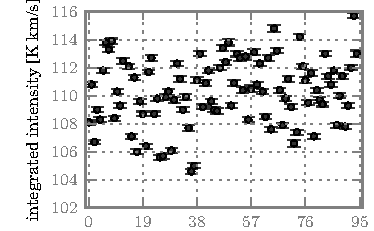
\includegraphics{spread_87_core_iint_corrected}&
            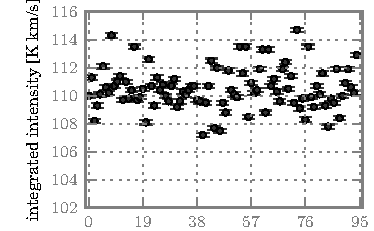
\includegraphics{spread_87_core_iint_noisy}    \\
            \bottomrule
        \end{tabular}
        \caption{
            Comparison of the \transition{CO}{8}{7} core component parameters
            for the real HIFI data (left column)
            and the synthetic noisy data (right column).
        }
        \label{fig:fit_core_87}
    \end{figure}
%    \clearpage
    \begin{figure}[p]
        \centering
        \begin{tabular}{@{}c@{}c@{}}
            \toprule
            \multicolumn{2}{c}{\transition{CO}{9}{8} core} \\
            diplexer-corrected & synthetic                 \\
            \midrule
            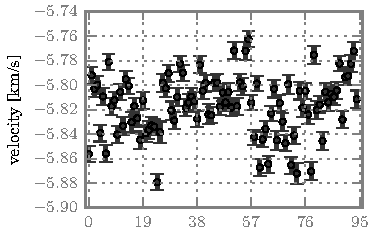
\includegraphics{spread_98_core_velo_corrected}&
            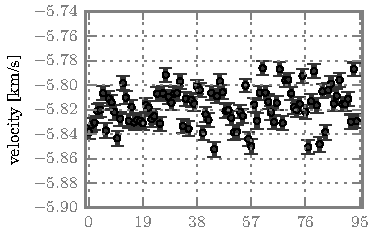
\includegraphics{spread_98_core_velo_noisy}    \\
            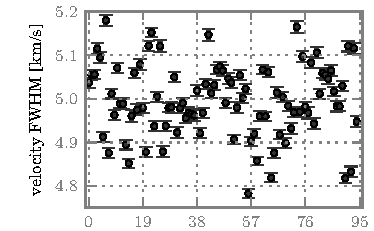
\includegraphics{spread_98_core_vfwh_corrected}&
            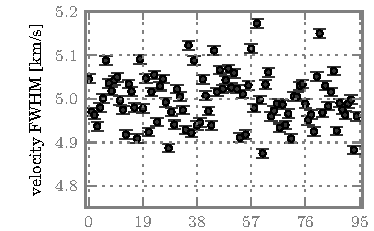
\includegraphics{spread_98_core_vfwh_noisy}    \\
            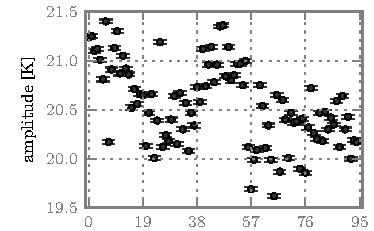
\includegraphics{spread_98_core_ampl_corrected}&
            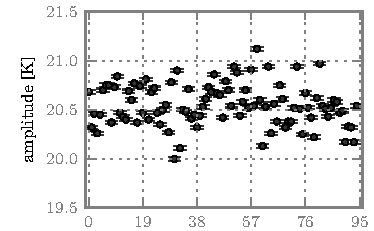
\includegraphics{spread_98_core_ampl_noisy}    \\
            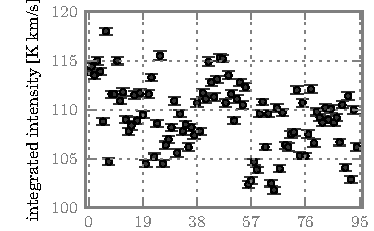
\includegraphics{spread_98_core_iint_corrected}&
            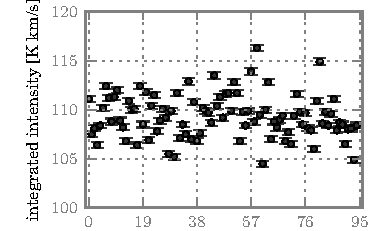
\includegraphics{spread_98_core_iint_noisy}    \\
            \bottomrule
        \end{tabular}
        \caption{
            Comparison of the \transition{CO}{9}{8} core component parameters
            for the real HIFI data (left column)
            and the synthetic noisy data (right column).
    }
        \label{fig:fit_core_98}
    \end{figure}
%    \clearpage
%    }%
%}

%\afterpage{% Make sure the two figures appear on even/odd pages for comparison.
%    \clearpage% flush all other floats
%    \ifodd\value{page}
%    %\else% uncomment this else to get odd/even instead of even/odd
%        \expandafter\afterpage% put it on the next page if this one is odd
%    \fi
%    {%
    \begin{figure}[p]
        \centering
        \begin{tabular}{@{}c@{}c@{}}
            \toprule
            \multicolumn{2}{c}{\transition{CO}{8}{7} outflow} \\
            diplexer-corrected & synthetic                 \\
            \midrule
            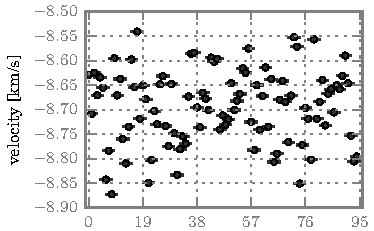
\includegraphics{spread_87_outf_velo_corrected}&
            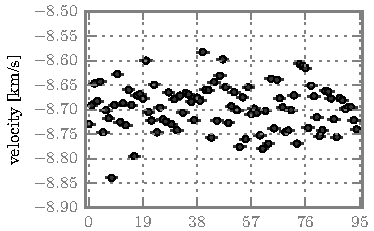
\includegraphics{spread_87_outf_velo_noisy}    \\
            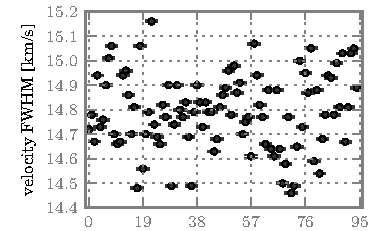
\includegraphics{spread_87_outf_vfwh_corrected}&
            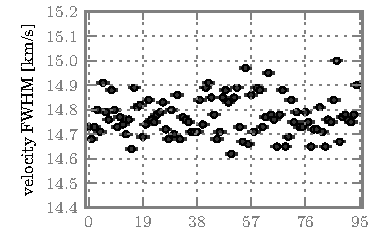
\includegraphics{spread_87_outf_vfwh_noisy}    \\
            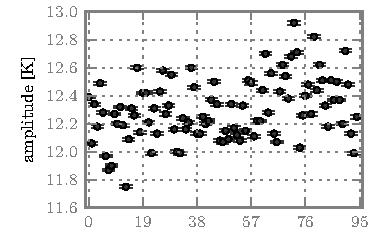
\includegraphics{spread_87_outf_ampl_corrected}&
            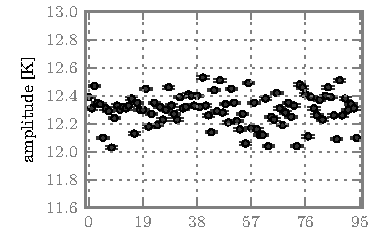
\includegraphics{spread_87_outf_ampl_noisy}    \\
            \includegraphics{spread_87_outf_iint_corrected}&
            \includegraphics{spread_87_outf_iint_noisy}    \\
            \bottomrule
        \end{tabular}
        \caption{
            Comparison of the \transition{CO}{8}{7} outflow component parameters
            for the real HIFI data (left column)
            and the synthetic noisy data (right column).
        }
        \label{fig:fit_outf_87}
    \end{figure}
%    \clearpage
    \begin{figure}[p]
        \centering
        \begin{tabular}{@{}c@{}c@{}}
            \toprule
            \multicolumn{2}{c}{\transition{CO}{9}{8} outflow} \\
            diplexer-corrected & synthetic                 \\
            \midrule
            \includegraphics{spread_98_outf_velo_corrected}&
            \includegraphics{spread_98_outf_velo_noisy}    \\
            \includegraphics{spread_98_outf_vfwh_corrected}&
            \includegraphics{spread_98_outf_vfwh_noisy}    \\
            \includegraphics{spread_98_outf_ampl_corrected}&
            \includegraphics{spread_98_outf_ampl_noisy}    \\
            \includegraphics{spread_98_outf_iint_corrected}&
            \includegraphics{spread_98_outf_iint_noisy}    \\
            \bottomrule
        \end{tabular}
        \caption{
            Comparison of the \transition{CO}{9}{8} outflow component parameters
            for the real HIFI data (left column)
            and the synthetic noisy data (right column).
        }
        \label{fig:fit_outf_98}
    \end{figure}
%    \clearpage
%    }%
%}

\begin{figure}
    \centering
    \begin{tabular}{@{}c@{}c@{}}
    \toprule
        \multicolumn{2}{c}{\transition{CO}{8}{7} self-absorption} \\
        diplexer-corrected & synthetic                 \\
    \midrule
        \includegraphics{spread_87_sabs_velo_corrected}&
        \includegraphics{spread_87_sabs_velo_noisy}    \\
        \includegraphics{spread_87_sabs_vfwh_corrected}&
        \includegraphics{spread_87_sabs_vfwh_noisy}    \\
        \includegraphics{spread_87_sabs_ampl_corrected}&
        \includegraphics{spread_87_sabs_ampl_noisy}    \\
        \includegraphics{spread_87_sabs_iint_corrected}&
        \includegraphics{spread_87_sabs_iint_noisy}    \\
    \bottomrule
    \end{tabular}
    \caption{
        Comparison of the \transition{CO}{8}{7} self-absorption component parameters for the real HIFI data (left column) and the synthetic noisy data (right column).
    }
    \label{fig:fit_sabs_87}
\end{figure}


%-----------------------------------------------------------------------------
\FloatBarrier
\subsubsection{Velocity-integrated intensity ratio}
\label{sec:line_ratios}
With 95 integrated intensities per transition, there are $95 \times 95 = 9025$ possible line ratios for the core and as many for the outflow.

We calculate the ratio of \transition{CO}{8}{7} over \transition{CO}{9}{8}.
We propagate the uncertainties using
\begin{equation}
    \frac{a \pm \sigma_a}{b \pm \sigma_b}
    =
    \frac{a}{b} \pm \frac{a}{b}\sqrt{(\sigma_a / a)^2 + (\sigma_b / b)^2}
    = c \pm \sigma_c
    \text{.}
\end{equation}
Each possible ratio has a normal distribution $c \pm \sigma_c$.
The sum of these 9025 distributions, divided by the number of distributions, is shown in \cref{fig:ratio_core,fig:ratio_outflow}.
The distribution of this ratio follows a normal curve.
The mean values and their uncertainties are given in \cref{tab:line_ratios}.
The calibration uncertainty is~\SI{4}{\percent} for the core and~\SI{2}{\percent} for the outflow.

The uncertainty on the synthetic ratios is~\SI{60}{\percent} that of the ratios measured on the real HIFI data.
If our noise model is correct, then \SI{40}{\percent} of the uncertainty on the line ratios is caused by non-thermal effects: interferences in the optics, intrinsic sideband ratio of the mixer or the unexplained~\SI{1.14}{\mega\hertz} ripple mentioned in~\cref{sec:noise_model_of_the_real_spectra}.
Longer integration times can reduce the uncertainty due to the noise, but have no effect on the remaining~\SI{2.4}{\percent} of systematic uncertainty on the core line ratio.

\vspace{5em}
\begin{table}[h]
%                        left      right    mean        -         +      fwhm
%    corrected    core   0.9615 .. 1.0546   1.0102   -0.0487   +0.0444   0.0931
%        noisy    core   0.9831 .. 1.0397   1.0113   -0.0282   +0.0285   0.0566
%    corrected outflow   0.9797 .. 1.0266   1.0029   -0.0232   +0.0236   0.0469
%        noisy outflow   0.9859 .. 1.0158   1.0016   -0.0158   +0.0142   0.0299
    \centering
    \begin{tabular}{lcc}
        \toprule
                & diplexer-corrected   & synthetic \\
        \midrule
        core    & $1.01 \pm 0.04$ & $1.01 \pm 0.02$ \\
        outflow & $1.01 \pm 0.02$ & $1.00 \pm 0.01$ \\
        \bottomrule
    \end{tabular}
    \caption{
        Velocity-integrated intensity ratios of
        \transition{CO}{8}{7} over \transition{CO}{9}{8}.
    }
    \label{tab:line_ratios}
\end{table}


\begin{figure}
    \centering
    \begin{subfigure}[0]{\textwidth}
        \centering
        \includegraphics[width=\textwidth]{ratios_core_corrected}
        \caption{Diplexer-corrected spectra;
        $\text{mean}=1.0102$, $\text{FWHM}=0.0931$, $\sigma=0.0395$.}
    \end{subfigure}
    \\
    \begin{subfigure}[0]{\textwidth}
        \centering
        \includegraphics[width=\textwidth]{ratios_core_noisy}
        \caption{Synthetic-noise spectra;
        $\text{mean}=1.0113$, $\text{FWHM}=0.0566$, $\sigma=0.0240$.}
    \end{subfigure}
    \caption{
        Core integrated intensity ratios for the real diplexer-corrected spectra (top)
        and the synthetic spectra (bottom).
    }
    \label{fig:ratio_core}
\end{figure}

\begin{figure}
    \centering
    \begin{subfigure}[0]{\textwidth}
        \centering
        \includegraphics[width=\textwidth]{ratios_outflow_corrected}
        \caption{Diplexer-corrected spectra;
        $\text{mean}=1.0029$, $\text{FWHM}=0.0469$, $\sigma=0.0199$.}
    \end{subfigure}
    \\
    \begin{subfigure}[0]{\textwidth}
        \centering
        \includegraphics[width=\textwidth]{ratios_outflow_noisy}
        \caption{Synthetic-noise spectra;
        $\text{mean}=1.0016$, $\text{FWHM}=0.0299$, $\sigma=0.0127$.}
    \end{subfigure}
    \caption{
        Outflow integrated intensity ratios for the real diplexer-corrected spectra (top)
        and the synthetic spectra (bottom).
    }
    \label{fig:ratio_outflow}
\end{figure}





%#############################################################################
\FloatBarrier
\section{\Radex{} modeling}



%=============================================================================
\subsection{Introduction and parameters}
In the previous section, we have derived the integrated intensity ratio of
\transition{CO}{8}{7} and \transition{CO}{9}{8} of S140~IRS1.
We use the computer program \radex{}%
\footnote{
    \Radex{} is publicly available at the following address:\\
    \url{http://www.sron.rug.nl/~vdtak/radex/index.shtml}.
}
to determine the volume number density and the kinetic temperature of~\ce{H2} from this line ratio.

\Radex{}~\parencite{vandertak2007radex} solves radiative transfer equations for a spherical homogeneous isothermal molecular cloud without large-scale velocity field.
\Radex{} does not assume Local Thermal Equilibrium~(LTE).
The LTE hypothesis states that the excitation temperature $T_\text{ex}$ and the kinetic temperature $T_\text{kin}$ are equal: the energy level population follows the Boltzmann distribution.
The LTE contition is rarely met in the interstellar medium where the densities are low:
the radiative decays compete with collisions and~$T_\text{ex}<T_\text{kin}$, a situation called ``subthermal excitation''~\parencite{vandertak2011radiative}.
For the level population, \radex{} assumes a statistical equilibrium: the sum of the collisional and radiative (de-)excitation rate for each level should be zero.
To solve the radiative transfer, \radex{} uses the escape-probability method first introduced by~\textcite{sobolev1960}.

\Radex{} computes the velocity-integrated intensity of molecular lines resulting from the collisions of a molecule (\ce{CO} for us) with a partner (\ce{H2} in our case).
In addition to tables describing the frequencies, Einstein coefficients, energy levels and collision rates of the molecular transitions, \radex{} requires the line width, the background radiation temperature, the kinetic temperature and volume number density of~\ce{H2}, and the abundance of~\ce{CO} given as a column density.
\Cref{tab:radex_input} lists the input parameters of our model.
\Radex{} calculates the default ortho/para spin ratio of~\ce{H2} by assuming that \transition{H2}{1}{0} is thermalized at the kinetic temperature.

\begin{table}
    \centering
    \begin{tabular}{lrl}
        \toprule
        parameter & value & unit \\
        \midrule
        molecule                         & \ce{^{12}C^{16}O} & \\
        collision partner                & \ce{H2}  & \\
        low frequency                    &  921.78  & \si{\giga\hertz} \\
        high frequency                   & 1036.91  & \si{\giga\hertz} \\
        ortho/para ratio of~\ce{H2}      & default  & \\
        background radiation temperature & 2.73     & \si{\kelvin}                \\
        line width (core)                &  4.98    & \si{\kilo\meter\per\second} \\
        line width (outflow)             & 14.34    & \si{\kilo\meter\per\second} \\
        \ce{H2} volume number density    & $10^{4.5}$ to $10^8$ & \si{\per\centi\meter\cubed} \\
        Kinetic temperature              & \numrange{20}{600}  & \si{\kelvin} \\
        \ce{CO} column density           & $10^{17}$ to $10^{19}$ & \si{\per\centi\meter\squared} \\
        \bottomrule
    \end{tabular}
    \caption{Parameters used in our \radex{} models.}
    \label{tab:radex_input}
\end{table}

For S140, a realistic number column density for \ce{CO} is~\SI{e19}{\per\centi\meter\squared}.
We also explore column densities of \num{e17} and \SI{e18}{\per\centi\meter\squared} which are realistic for \ce{C^{18}O} and \ce{^{13}CO}, respectively.

\Radex{} takes a single line width for the two transitions.
We set it to the average of the two line widths, which is not a problem for the core component but less justified for the outflow where they differ by~\SI{6}{\percent}
(see~\cref{tab:line_widths}).

\begin{table}
    % Linewidth
    % Corrected data:
    %     87 core 4.95989473684 +/- 0.0678930232342
    %     98 core 4.99625263158 +/- 0.0818054133354
    %     87 outf 14.7908421053 +/- 0.152892553658
    %     98 outf 13.8824210526 +/- 0.254130988974
    % Noisy (synthetic noise):
    %     87 core 4.96398947368 +/- 0.049699622944
    %     98 core 4.99835789474 +/- 0.0585537837852
    %     87 outf 14.7727368421 +/- 0.0790262062498
    %     98 outf 13.8842105263 +/- 0.126104208765
    %
    % Error propagation on a sum:
    %     c = a + b
    %     dc = sqrt(da^2+db^2)
    % I use that to compute the average of the linewidths that I can feed to RADEX.
    %
    % Corrected:
    %     avg core  4.97807368421 +/- 0.05315446419364808
    %     avg outf 14.33663157895 +/- 0.1482891537849007
    % Noisy:
    %     avg core  4.98117368421 +/- 0.038401165725599144
    %     avg outf 14.3284736842  +/- 0.0744100341729572
    \centering
    \begin{tabular}{lrrrr}
        \toprule
                & \transition{CO}{8}{7} & \transition{CO}{9}{8} &
                \multicolumn{1}{c}{average} &
                \multicolumn{1}{c}{$\abs{\text{difference}}$} \\
        \midrule
        core    & $ 4.96 \pm 0.07$  & $ 5.00 \pm 0.08$  & $ 4.98 \pm 0.05$ & $0.04 \pm 0.11$\\
        outflow & $14.79 \pm 0.15$  & $13.88 \pm 0.25$  & $14.34 \pm 0.15$ & $0.91 \pm 0.30$\\
        \bottomrule
    \end{tabular}
    \caption{
        Line widths (\textsc{fwhm}) in \si{\kilo\meter\per\second} of the core and outflow components of
        \transition{CO}{8}{7} and \transition{CO}{9}{8}.
    }
    \label{tab:line_widths}
\end{table}



%=============================================================================
\FloatBarrier
\subsection{Results}
\Cref{fig:radex_core,fig:radex_outf} present the line ratios that \radex{} predicts as a function of the temperature and density of~\ce{H2} for several column densities of~{CO}.
The contours follow the mean and the full-width at half-maximum of the line ratio distributions derived in~\cref{sec:line_ratios}:
the outer contours correspond to the total uncertainty and the inner contours to the thermal-noise uncertainty only.

\begin{figure}
    \centering
    \begin{tabular}{cc}
        \toprule
        $N_\ce{CO}$ [\si{\per\centi\meter\squared}]
        &
        core velocity-integrated intensity ratio
        \\
        \midrule
        $10^{17}$ &
        \begin{minipage}{9.5cm}
            \includegraphics[width=\linewidth]{radex_grid_core_n170_t00273}
        \end{minipage}
        \\
        $10^{18}$ &
        \begin{minipage}{9.5cm}
            \includegraphics[width=\linewidth]{radex_grid_core_n180_t00273}
        \end{minipage}
        \\
        $10^{19}$ &
        \begin{minipage}{9.5cm}
            \includegraphics[width=\linewidth]{radex_grid_core_n190_t00273}
        \end{minipage}
        \\
        \bottomrule
    \end{tabular}%
    \caption{\Radex{} predictions of the integrated intensity line ratio \transition{CO}{8}{7}/\transition{CO}{9}{8} in the core of IRS1 as a function of the volume number density of molecular hydrogen and its kinetic temperature, for four column densities of~\ce{CO}.}
    \label{fig:radex_core}
\end{figure}


\begin{figure}
    \centering
    \begin{tabular}{cc}
        \toprule
        $N_\ce{CO}$ [\si{\per\centi\meter\squared}]
        &
        outflow velocity-integrated intensity ratio\\
        \midrule
        $10^{17}$ &
        \begin{minipage}{9.5cm}
            \includegraphics[width=\linewidth]{radex_grid_outf_n170_t00273}
        \end{minipage}
        \\
        $10^{18}$ &
        \begin{minipage}{9.5cm}
            \includegraphics[width=\linewidth]{radex_grid_outf_n180_t00273}
        \end{minipage}
        \\
        $10^{19}$ &
        \begin{minipage}{9.5cm}
            \includegraphics[width=\linewidth]{radex_grid_outf_n190_t00273}
        \end{minipage}
        \\
        \bottomrule
    \end{tabular}%
    \caption{\Radex{} predictions of the integrated intensity line ratio \transition{CO}{8}{7}/\transition{CO}{9}{8} in the outflow of IRS1 as a function of the volume number density of molecular hydrogen and its kinetic temperature, for four column densities of~\ce{CO}.}
    \label{fig:radex_outf}
\end{figure}

In all cases, a line ratio of~\num{1.01} indicates temperatures above~\SI{200}{\kelvin}.
This result could be predicted simply by considering that the upper-level energies
of~\transition{CO}{8}{7} and \transition{CO}{9}{8} are~\SI{200}{\kelvin} and~\SI{250}{\kelvin} (\cref{table:co_transition_frequencies}).
This confirms the assumption that we made in~\cref{sec:s140irs1} regarding the angular size of the emitting region: 
we seem to be probing a warm region of the molecular cloud, a region close to the young stellar object at the center of IRS1.

In addition to a lower-limit on the temperature, these plots give a lower-limit of the density: $n_\ce{H2} > \SI{e5}{\per\centi\meter\cubed}$.
According to~\textcite{goldsmith2001}, at densities above $10^{4.5} \si{\per\centi\meter\cubed}$, the dust and the gas are collisionally coupled.
This suggests that the dust temperature is also of the order of~\SI{200}{\kelvin} in that region, in which case out background temperature of~\SI{273}{\kelvin} may be underestimated.
We have run our \radex{} analysis with background temperatures up to~\SI{100}{\kelvin} and confirmed that the influence of the background temperature on the interpretation of our line ratio is negligible.

For number volume densities of \ce{H2} above~\SI{e6}{\per\centi\meter\cubed}, our line ratio can constitute a useful tracer of temperature.
For low ($<10^{18}$) number column densities of \ce{CO}, the uncertainty on the line ratio translates linearly into an uncertainty on the temperature (although the distribution may be skewed).
However, this same uncertainty makes it absolutely unusable at higher column densities.



%=============================================================================
\FloatBarrier
\subsection{Discussion}

The number column density of~\ce{CO} in the direction of S140 IRS1 has been estimated to~\SI{3e19}{\per\centi\meter\squared}~\parencite{poelman2006line,koumpia2015}.
In this domain, the lines of~\transition{CO}{8}{7} and~\transition{CO}{9}{8} are optically thick, as evidenced by the self-absorption feature observed on the line profile in~\cref{fig:spectra_transitions}.
\Radex{} does not take into account the variation of optical depth along the profile of the line \parencite{langevelde2004} which makes these lines sub-optimal for the study of~S140~IRS1 with \radex{}.
In order to continue their study one should use more detailed models (see \cite{zadelhoff2002} for a list), which often converge much slower.

A recent study \parencite{koumpia2015} using techniques similar to ours (\radex{} modeling of HIFI spectra of \transition{CO}{9}{8}, \transition{C^{18}O}{9}{8} and~\transition{^{13}CO}{10}{9} of S140~IRS1) concludes that the temperature of the gas is approximately~\SI{50}{\kelvin} near the core.
This contrasts with our lower-limit estimate of~\SI{200}{\kelvin}.
One explanation for this discrepancy is that this study involves low-$J$ \ce{CO} lines: the kinetic temperature of~\SI{50}{\kelvin} is derived from the ratios of~\transition{CO}{1}{0} and~\transition{CO}{2}{1}, and the higher-$J$ data provides additional constraints.
With upper-energy levels of~\num{5.53} and~\SI{16.6}{\kelvin}, \transition{CO}{1}{0} and~\transition{CO}{2}{1} are visible in cold regions of the cloud, far away from its hot central object, their emission fills the beam.
Combining high and low-$J$ transitions without modeling the temperature gradient can result in a slightly over-estimated large-scale temperature (a minor concern for their study) or a greatly under-estimated temperature of the small-scale core.

If we compare our observation to the PDR model presented in the same article (spherical PDR, inner-radius $n_\ce{H2}=\SI{e5}{\per\centi\meter\cubed}$, radiation of~100~Drain fields), we find that our temperature of~\SI{200}{\kelvin} originates within~\SI{20}{\astronomicalunit} of the central star.
This places us near the inner radius of the accretion disk~\parencite{maud2013resolving}.

More detailed PDR models can take into account the clumpy nature of S140 reported by~\textcite{poelman2006line}.
This is a refinement over the simple gradient of temperature: there are regions of lower density which allow the UV radiation to penetrate farther into the molecular cloud, creating hotter regions at a greater distance from the core.

An alternative to complex models is to keep using \radex{} with other transition lines.
Isotopes of~\ce{CO} such as \ce{^{13}CO} or \ce{C^{18}O} are less abundant than \ce{CO}.
Consequently their lines can remain optically thin even at high column densities, allowing~\radex{} to perform more optimally.
However, a lower abundance also implies a lower signal-to-noise ratio and therefore a longer integration time.
That longer integration time would certainly lower the noise but would have no effect on the modulation of the optical gain of the detector by interferences; one would trade a well known uncertainty for another, much more difficult to handle.


%#############################################################################
\FloatBarrier
\section{Conclusion}
We observed S140 IRS1 with HIFI and measured the intensities of its~\transition{CO}{8}{7} and \transition{CO}{9}{8} lines.
The line profiles show evidence two sources of emission:
a core and an outflow.

Each line was observed 95 times, with 95 different optical configurations of HIFI.
The optical configuration influences the line profiles.
A statistical analysis of these 190 spectra allowed us to compute the uncertainties on the line velocity-integrated intensity ratios of \transition{CO}{8}{7} over \transition{CO}{9}{8}.
The ratio is $1.01 \pm 0.04$ for the core and $1.01 \pm 0.02$ for the outflow.

In order to quantify the uncertainties due to the thermal noise and that due to non-thermal effects such as interferences in the optical cavities of HIFI, we modeled the thermal noise and created synthetic spectra.
The line ratios measured on these synthetic spectra have a smaller uncertainty than the line ratios measured on the real spectra.
In our study, only \SI{60}{\percent} of the uncertainty on the line ratio is due to thermal effects; the remaining \SI{40}{\percent} have a systematic origin.
The systematic uncertainty on our line ratios is~\SI{2.4}{\percent}.

Sources of systematic uncertainties include
interferences in the optics,
an intrinsic sideband gain imbalance of the mixer
and an unexplained~\SI{1.4}{\mega\hertz} oscillation of the baseline.
We lacked the signal-to-noise, the spectral resolution and the number of equations to properly constrain the many free parameters of an interference model of HIFI.
Nevertheless, we have shown that even low coefficients of reflection are sufficient to explain all the systematic uncertainty that we observed.

The lines that we observed are narrow ($< \SI{100}{\mega\hertz}$), of the order of the period of the shortest ripple ($\approx~\SI{90}{\mega\hertz}$) caused by interferences in HIFI.
In consequence, the ripples are almost undetectable on these spectra, they do not create clear sinusoidal distortions of the line profile, they merely shift the amplitude or velocity of the line.
The continuum being low, its modulation by interferences is drown in the noise.
Consequently, the spectra show no obvious evidence of being affected by interferences
and the astronomer could be mislead into trusting the measurement beyond the irreducible~\SI{2.4}{\percent} of accuracy.

We used \radex{} to predict the line ratios that we expect from a molecular cloud as a function of its density, kinetic temperature and \ce{CO} abundance.
In the specific case of S140 IRS1, the lines of \transition{CO}{8}{7} and \transition{CO}{9}{8} are optically thick, which makes this line ratio useless as a tracer of temperature or density.
However, if the column density of \ce{CO} were lower, the uncertainty on the line ratio would translate almost linearly into an uncertainty on the gas kinetic temperature.

Despite these uncertainties, we estimate that the emission of \transition{CO}{8}{7} and \transition{CO}{9}{8} in S140 IRS1 originates from a warm ($T_\text{kin}> \SI{200}{\kelvin}$) and dense ($n_\ce{H2} > \SI{e5}{\per\centi\meter\cubed}$) region,
possibly within~\SI{20}{\astronomicalunit} of the young stellar object if we neglect the clumpiness of the cloud, but not from the accretion disk itself.


%#############################################################################
\section*{Acknowledgements}
I would like to thank my many supervisors for their suggestions, support and feedback during the writing of this chapter.
In no particular order:
John Pearson, who suggested using S140 to constrain the imaginary part of the reflection coefficients in the HIFI FPU;
Floris van der Tak, whose familiarity with S140 and \radex{} made him indispensable all along;
Marc Verheijen, whose astronomical expertise is related but different, allowing him to evaluate my work from a more objective point of view;
and finally Peter Roelfsema, who on many occasion helped me bridge the gap between engineering and astronomy.

In addition, I especially wish to express my gratitude to David Teyssier, who wrote the non-standard observing mode that we use in our observations;
to Ian Avruch, who worked under a high time pressure to set up the specific observation parameters and submit them to the Mission Operation Center for the last calibration campaign of the HIFI mission;
and to Evgenia Koumpia, for her expertise of S140 which kept my data analysis on the right track.
%#############################################################################
%\clearpage
%\printbibliography[heading=subbibliography]
%\end{refsection}
